%!TEX root = ../main.tex

\chapter{View}
\label{chap:view}


\section{Haupseite und Buchung}

Das Mockup der Startseite der Anwendung ist in \ref{fig:startseite} dargestellt.

Die entsprechende implementierte Startseite wird gezeigt in \ref{fig:impl-startseite_lightmode},
dabei ist zu beachten, dass wir neben einen \textit{Light Mode} auch einen \textit{Dark Mode} implementiert haben,
welcher beispielhaft für die \textit{Kalender} Ansicht in \ref{fig:impl-startseite} zu sehen ist.
Im Folgenden werden wir zur besseren Erkenntlichkeit im Dokument immer die Bilder der Implementation im \textit{Light Mode}
verwenden.

Der Wechsel zwischen den beiden Modi ist über die Browser-Einstellungen möglich.

\begin{figure}[ht]
    \centering
    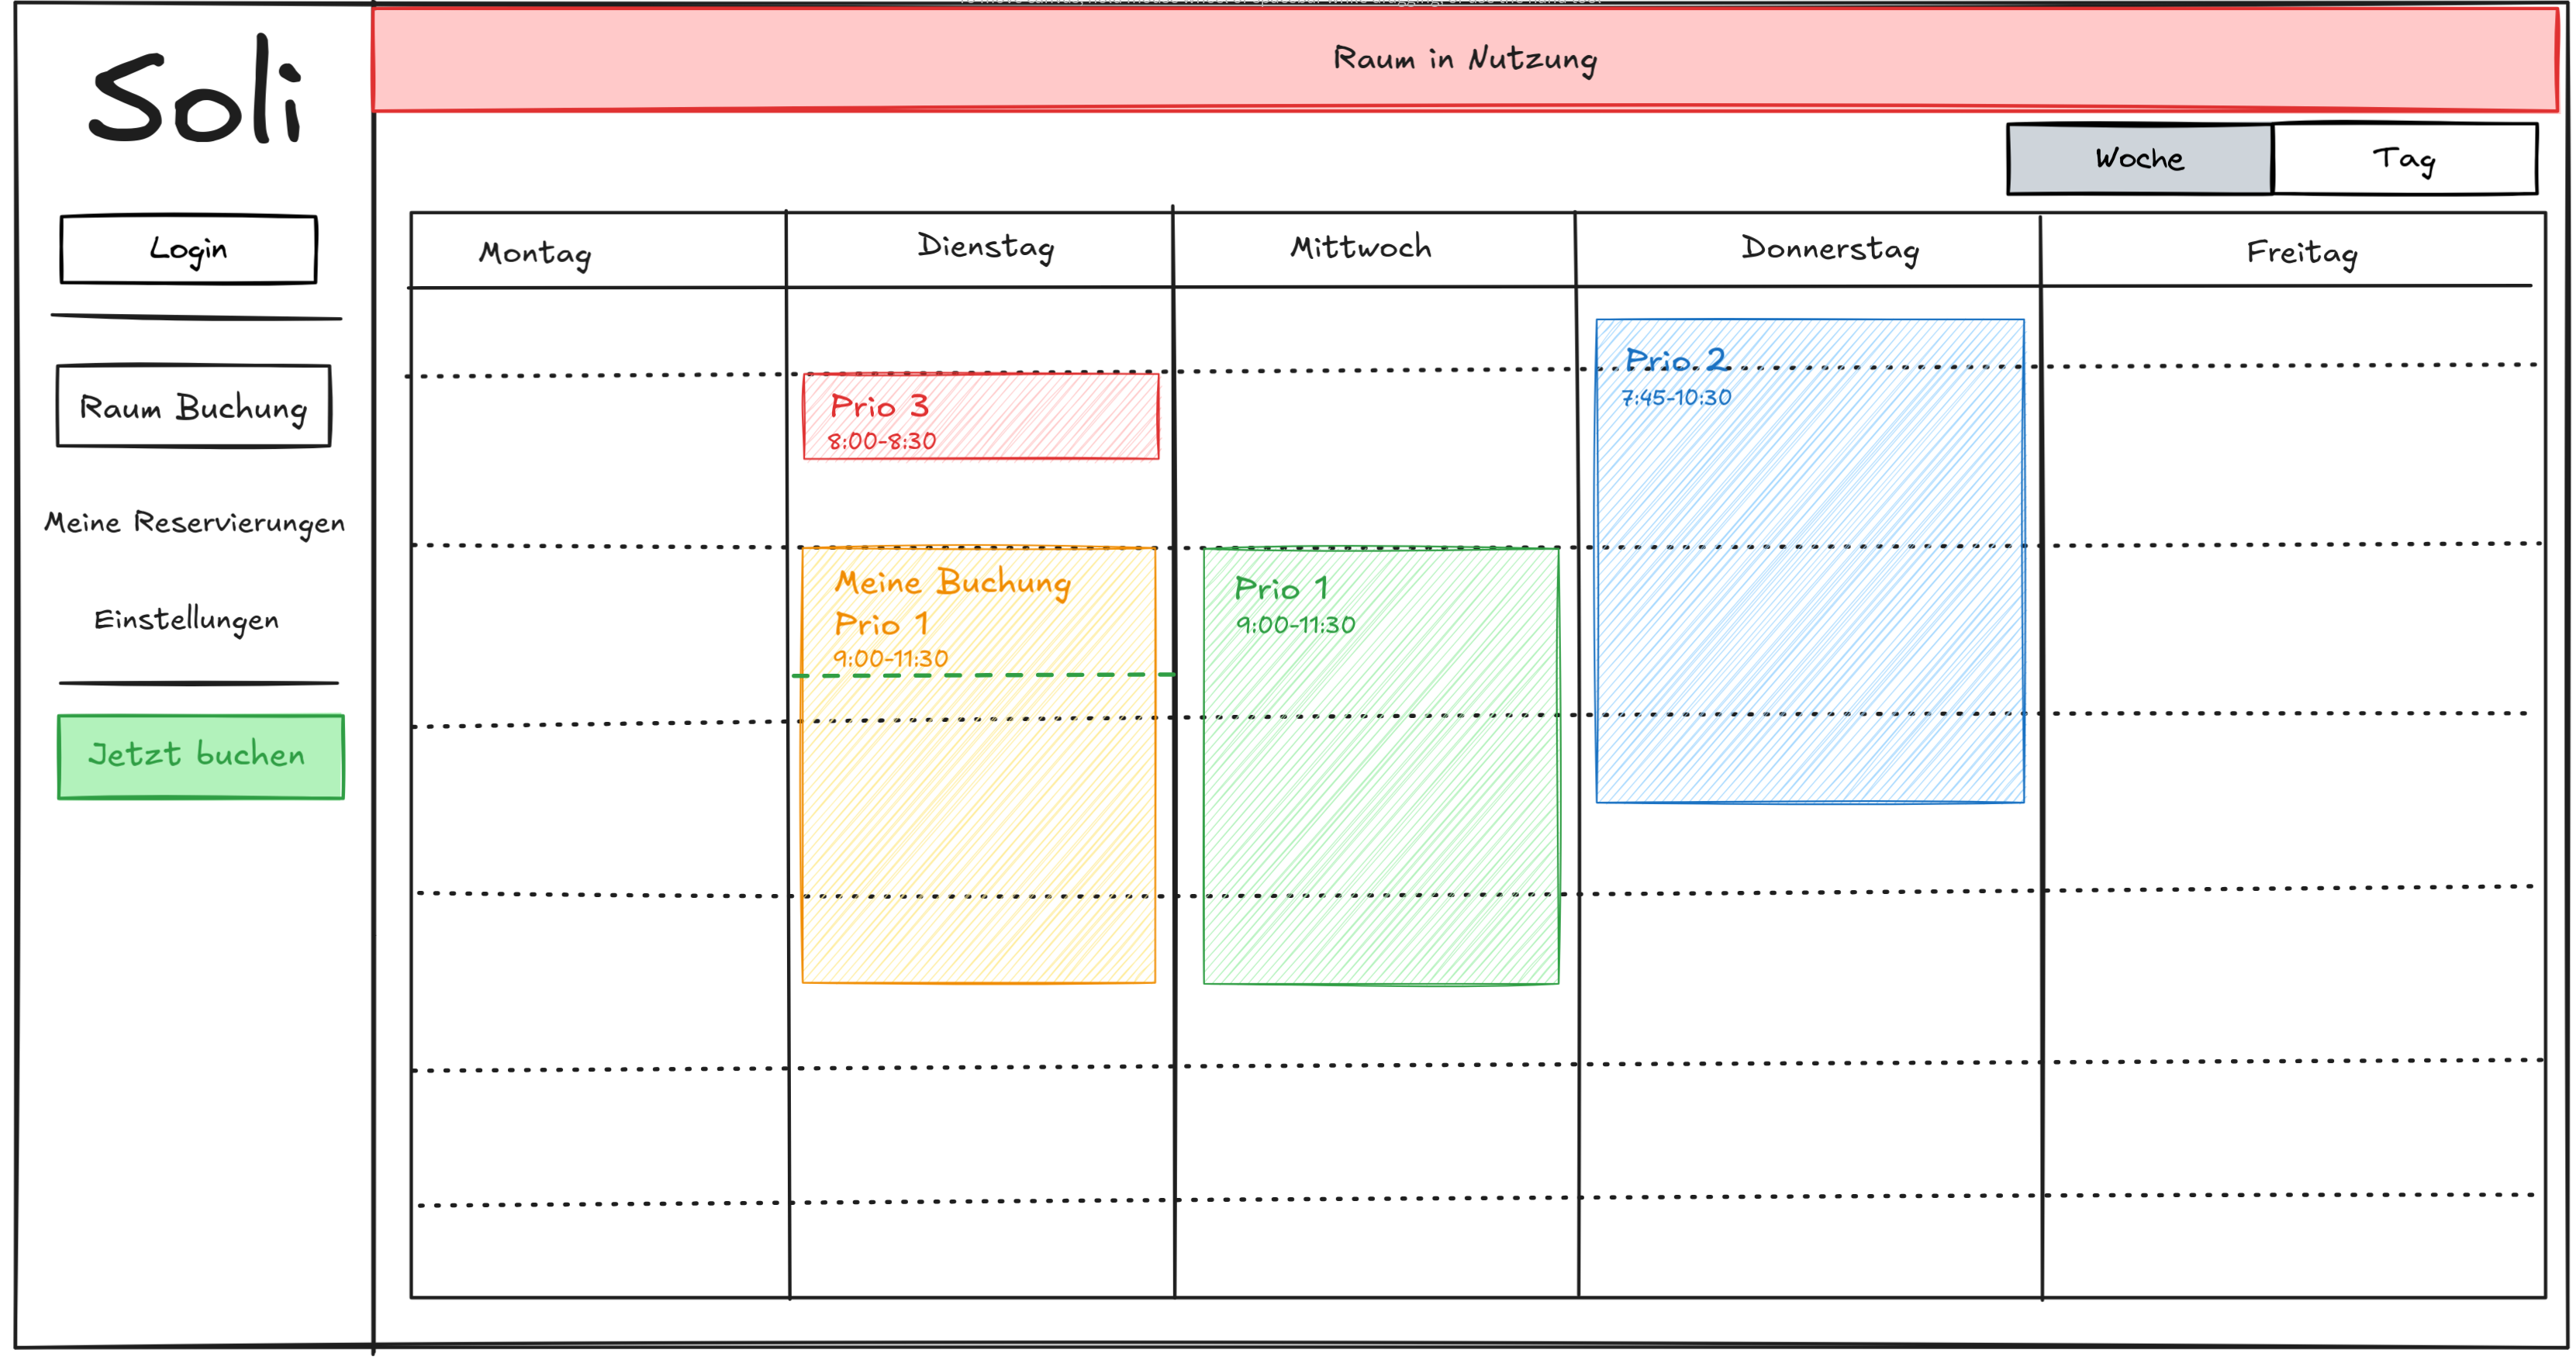
\includegraphics[width=\textwidth]{figures/mockup/calendar}
    \caption{Startseite der Anwendung}
    \label{fig:startseite}
\end{figure}
\pagebreak

\begin{figure}[ht]
    \centering
    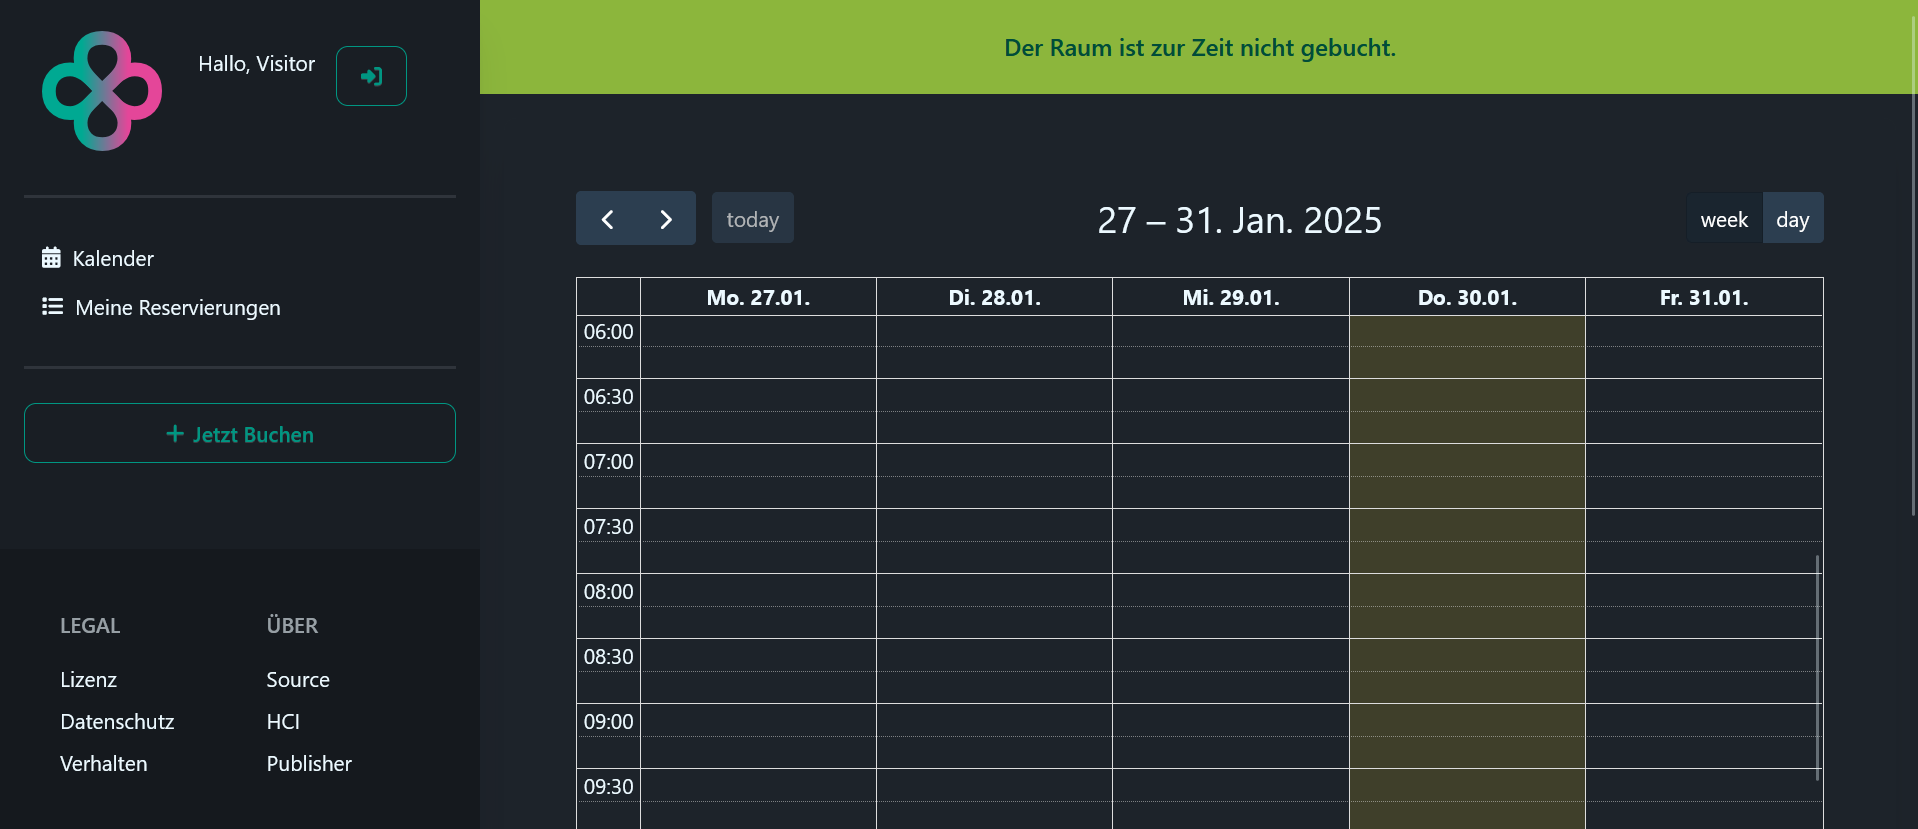
\includegraphics[width=\textwidth]{figures/impl-views/calendar_dark}
    \caption{Implementierung: Startseite der Anwendung}
    \label{fig:impl-startseite}
\end{figure}
\begin{figure}[ht]
    \centering
    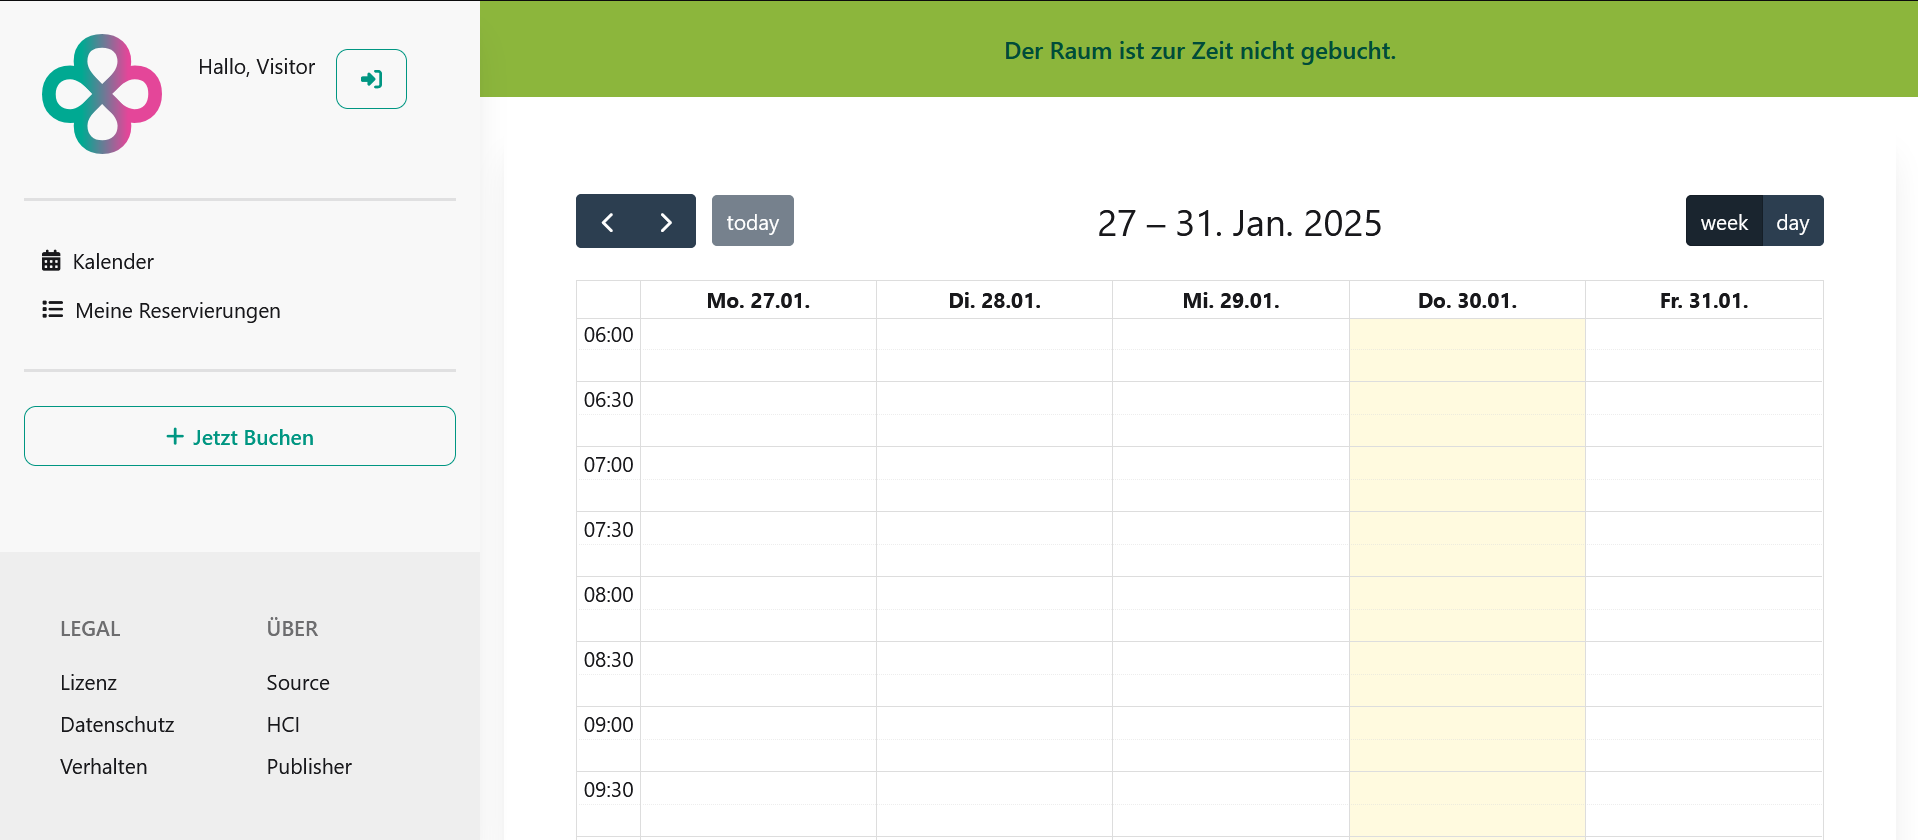
\includegraphics[width=\textwidth]{figures/impl-views/calendar_light}
    \caption{Implementierung: Startseite der Anwendung im Lightmode}
    \label{fig:impl-startseite_lightmode}
\end{figure}
\pagebreak

Sollten Nutzende eine Buchung vornehmen wollen, so klicken diese in den gewünschten Zeitraum
und es wird der Dialog in \ref{fig:buchung} dargestellt.

Der Dialog bietet Nutzenden die Möglichkeit, den genauen Start- und Endzeitpunkt des Termins festzulegen.

Außerdem können Nutzende die Priorität des Termins als \textit{Niedrig}, \textit{Mittel} oder \textit{Hoch} angeben.
Nutzende können auch bestimmen, ob sie bereit sind, den Raum mit anderen Nutzenden zu teilen.
Für diesen Zweck werden Ihnen drei Optionen bereitgestellt: \textit{Ja}, \textit{Nein} und \textit{Auf Anfrage}.

Letztlich können Nutzende eine Beschreibung für den Termin hinterlegen, die anderen angemeldeten Nutzenden angezeigt wird.

Die Implementierung des Dialogs ist in \ref{fig:impl-buchung1} und \ref{fig:impl-buchung2} zu sehen.

\begin{figure}[ht]
    \centering
    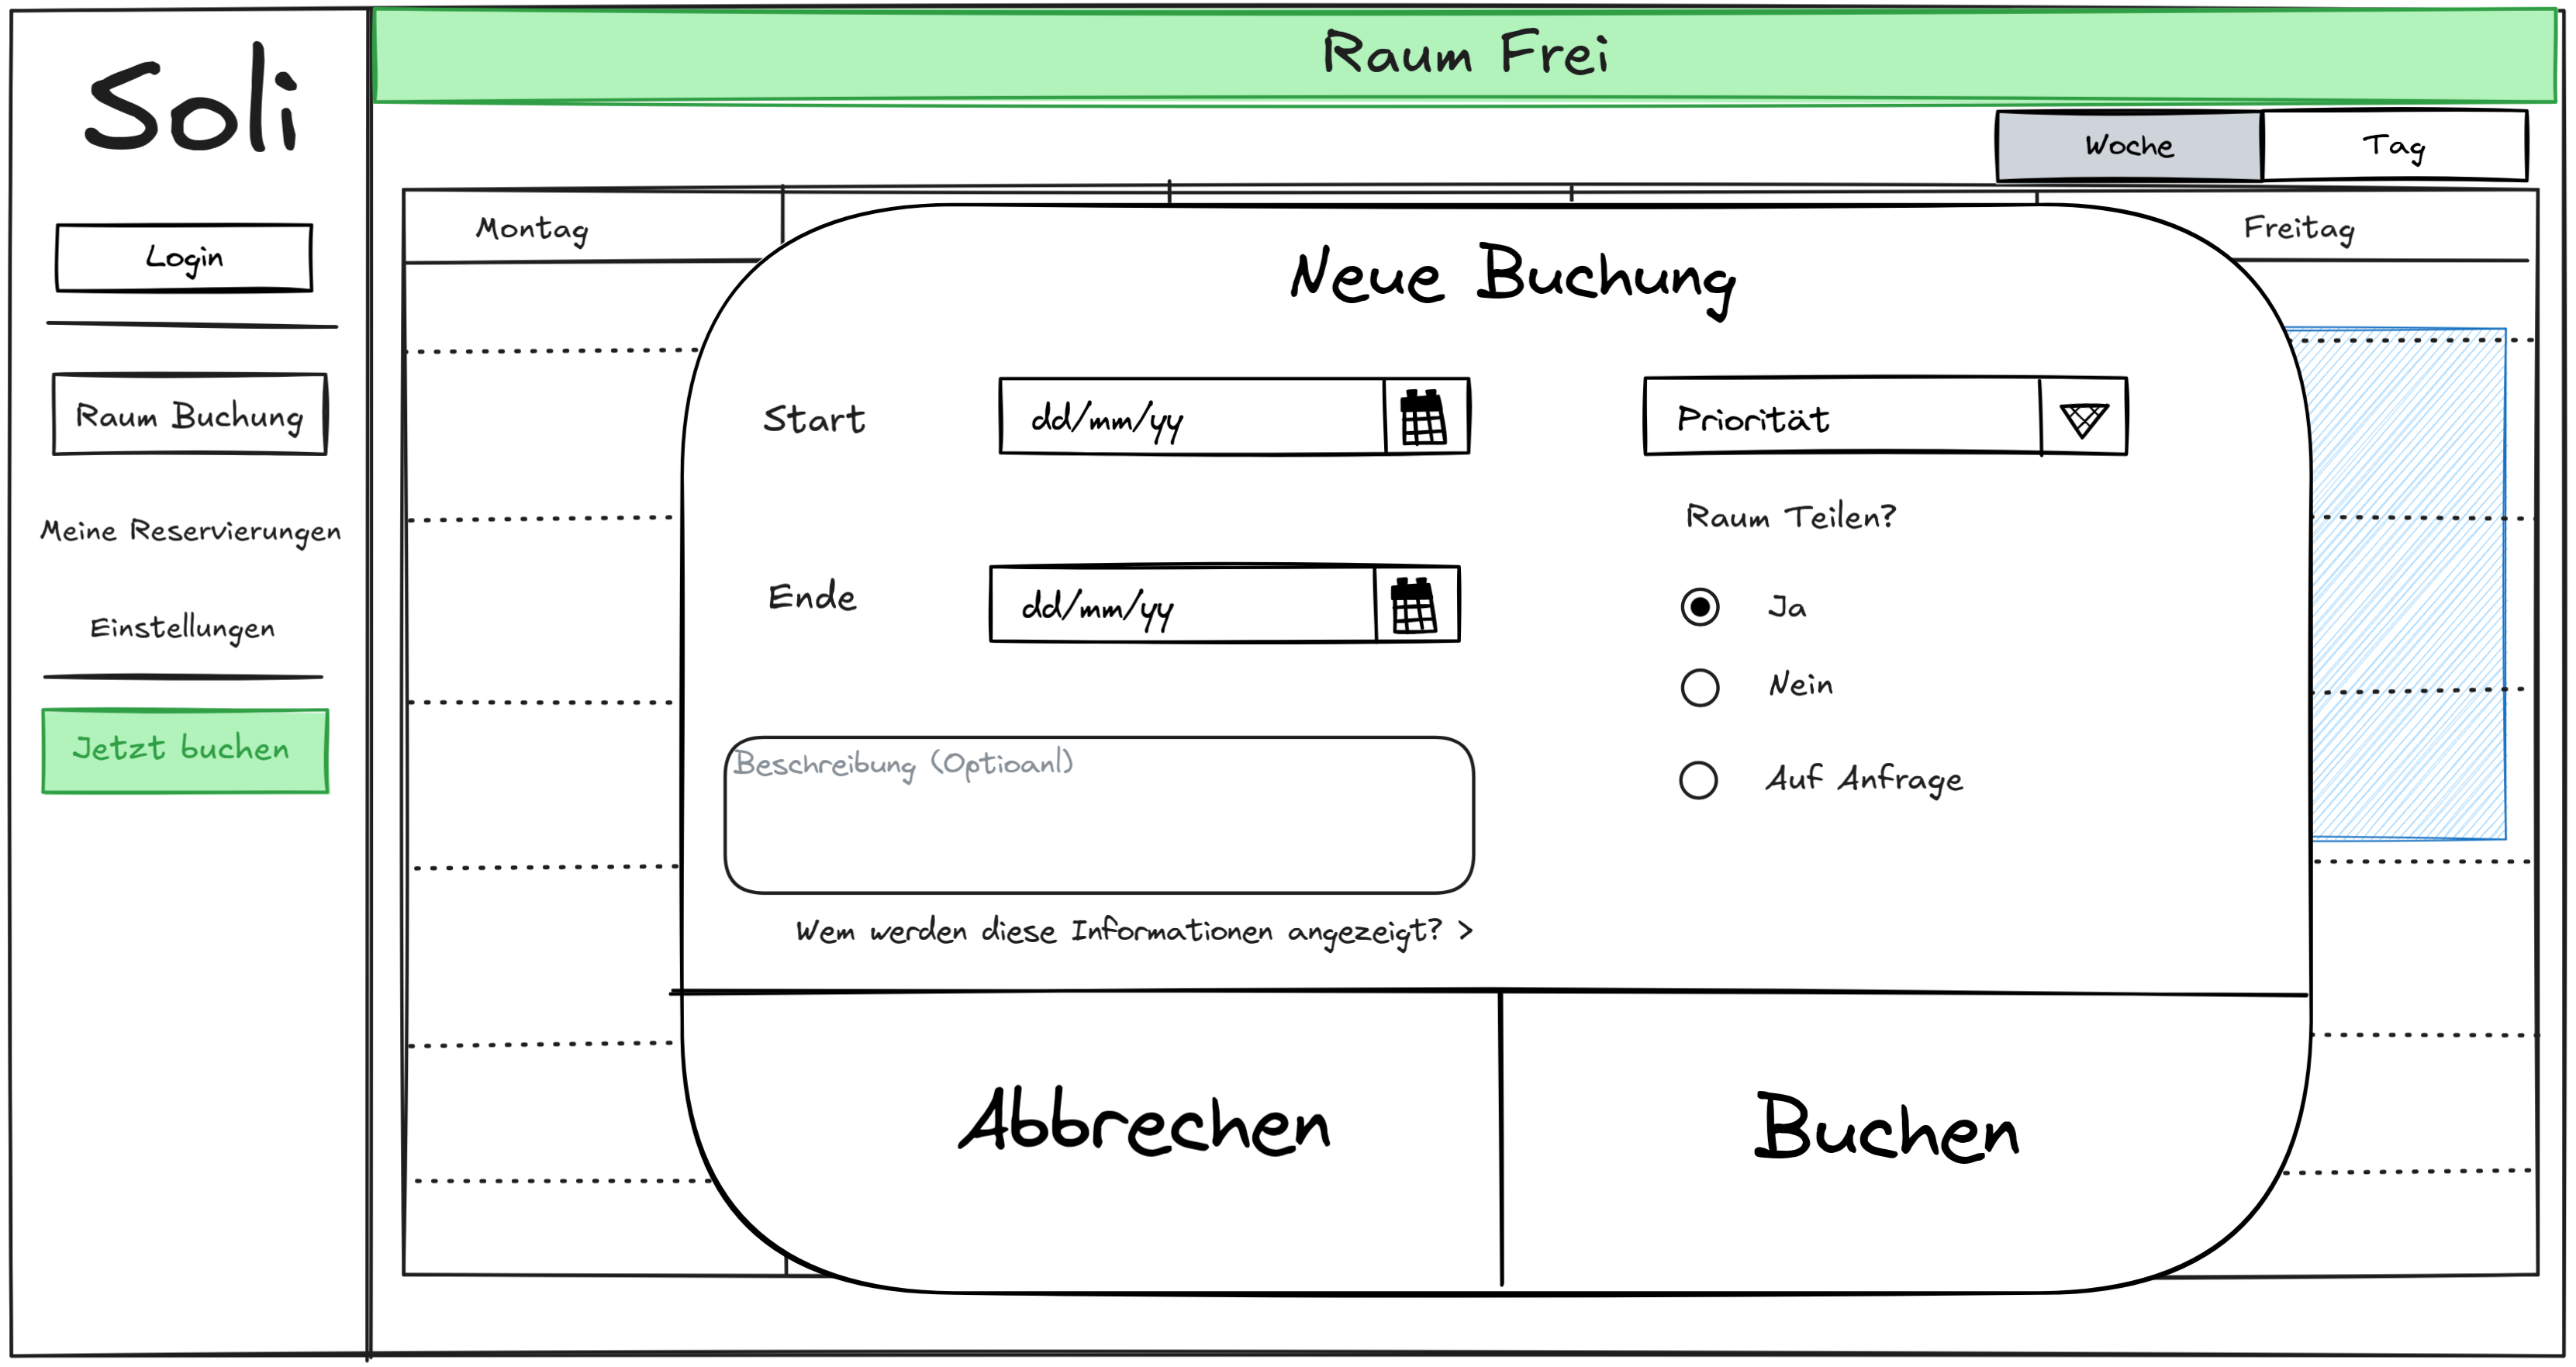
\includegraphics[width=\textwidth]{figures/mockup/bookings_create_form}
    \caption{Termin-erstellen}
    \label{fig:buchung}
\end{figure}
\pagebreak

\begin{figure}[ht]
    \centering
    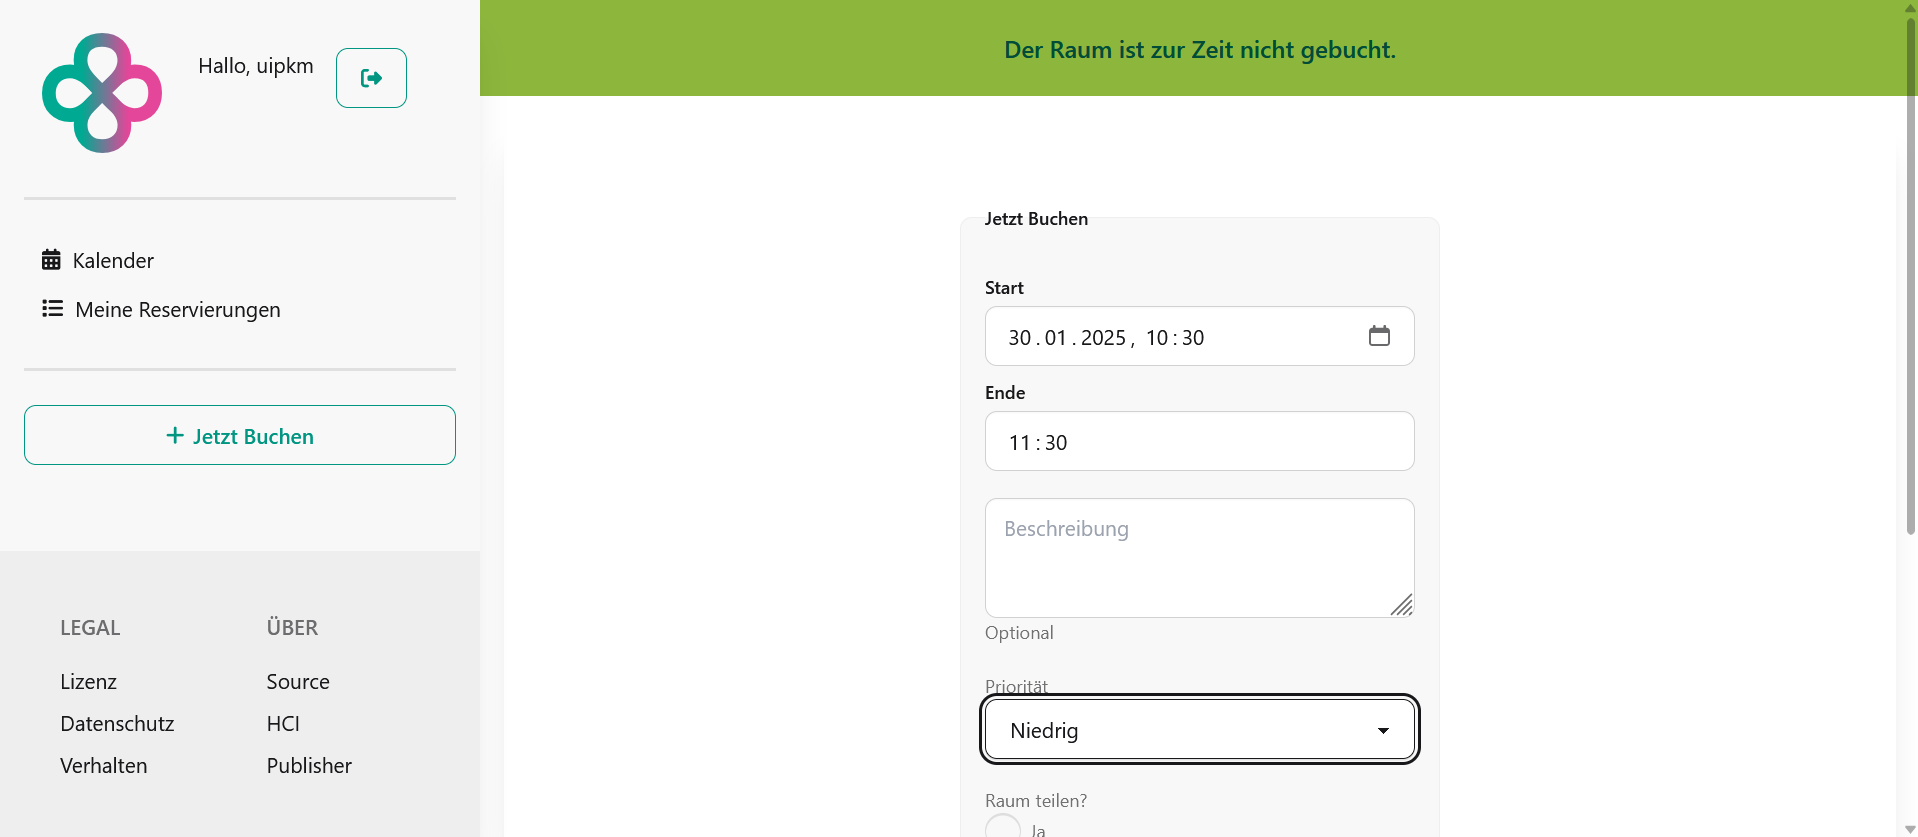
\includegraphics[width=\textwidth]{figures/impl-views/book1_light}
    \caption{Implementierung: Termin-erstellen}
    \label{fig:impl-buchung1}
\end{figure}

\begin{figure}[ht]
    \centering
    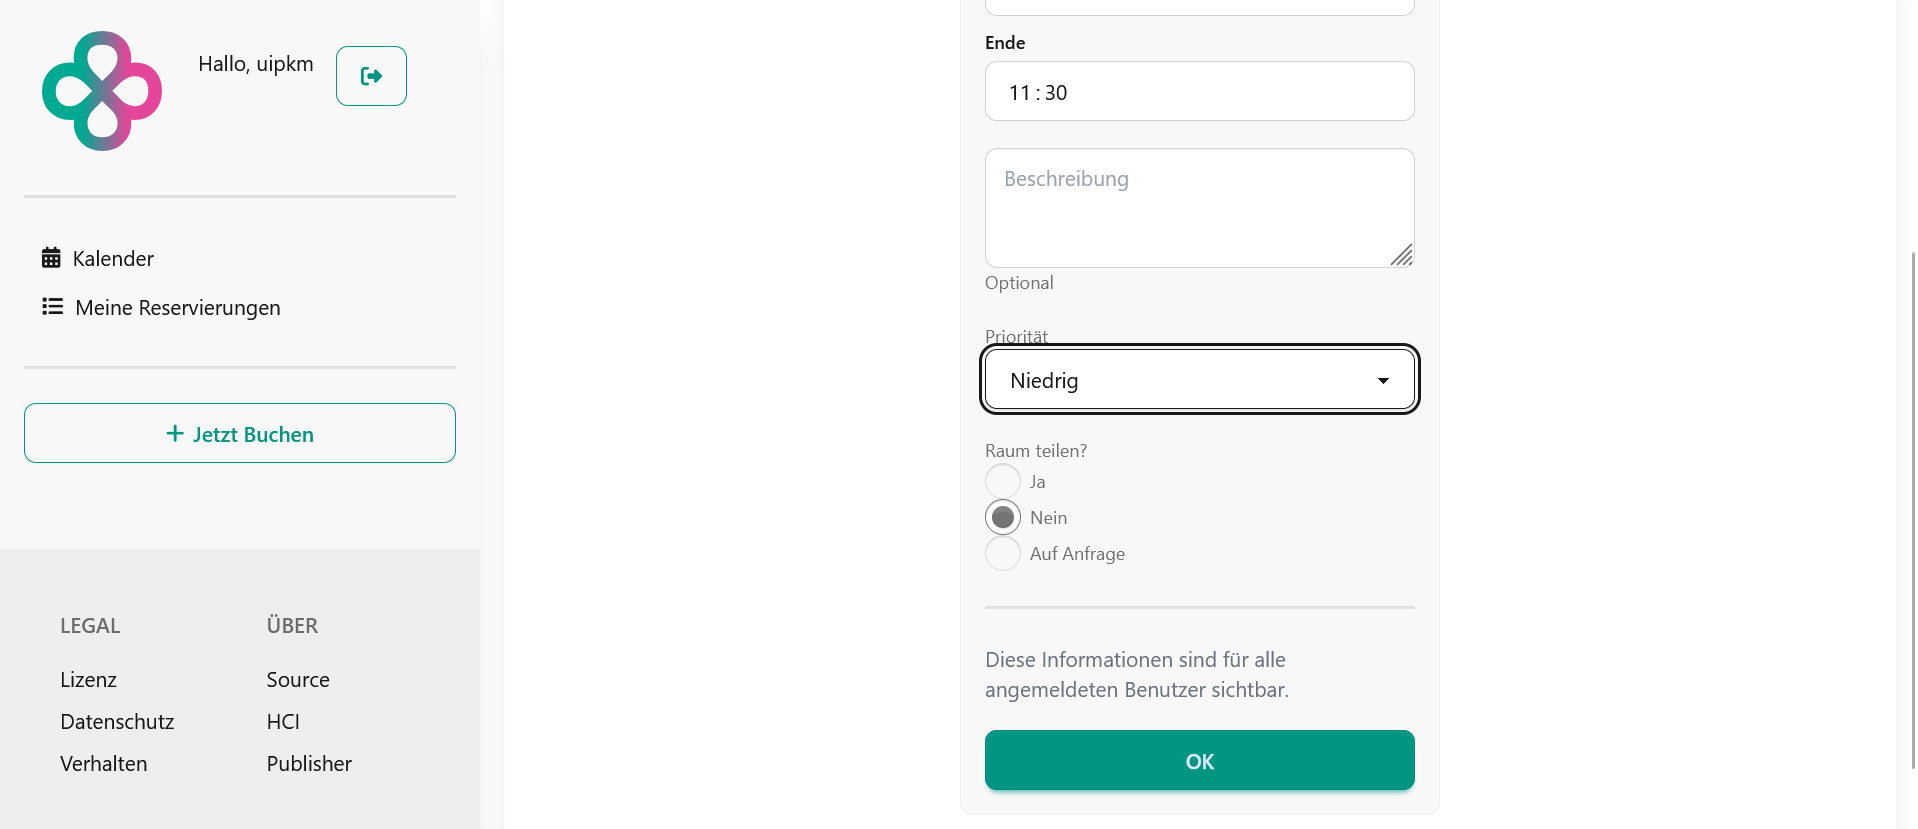
\includegraphics[width=\textwidth]{figures/impl-views/book2_light}
    \caption{Implementierung: Termin-erstellen}
    \label{fig:impl-buchung2}
\end{figure}
\clearpage

In \ref{fig:login} ist die Anmeldungsansicht dargestellt und in \ref{fig:impl-login} ist die tatsächliche Implementierung zu sehen.

\begin{figure}[ht]
    \centering
    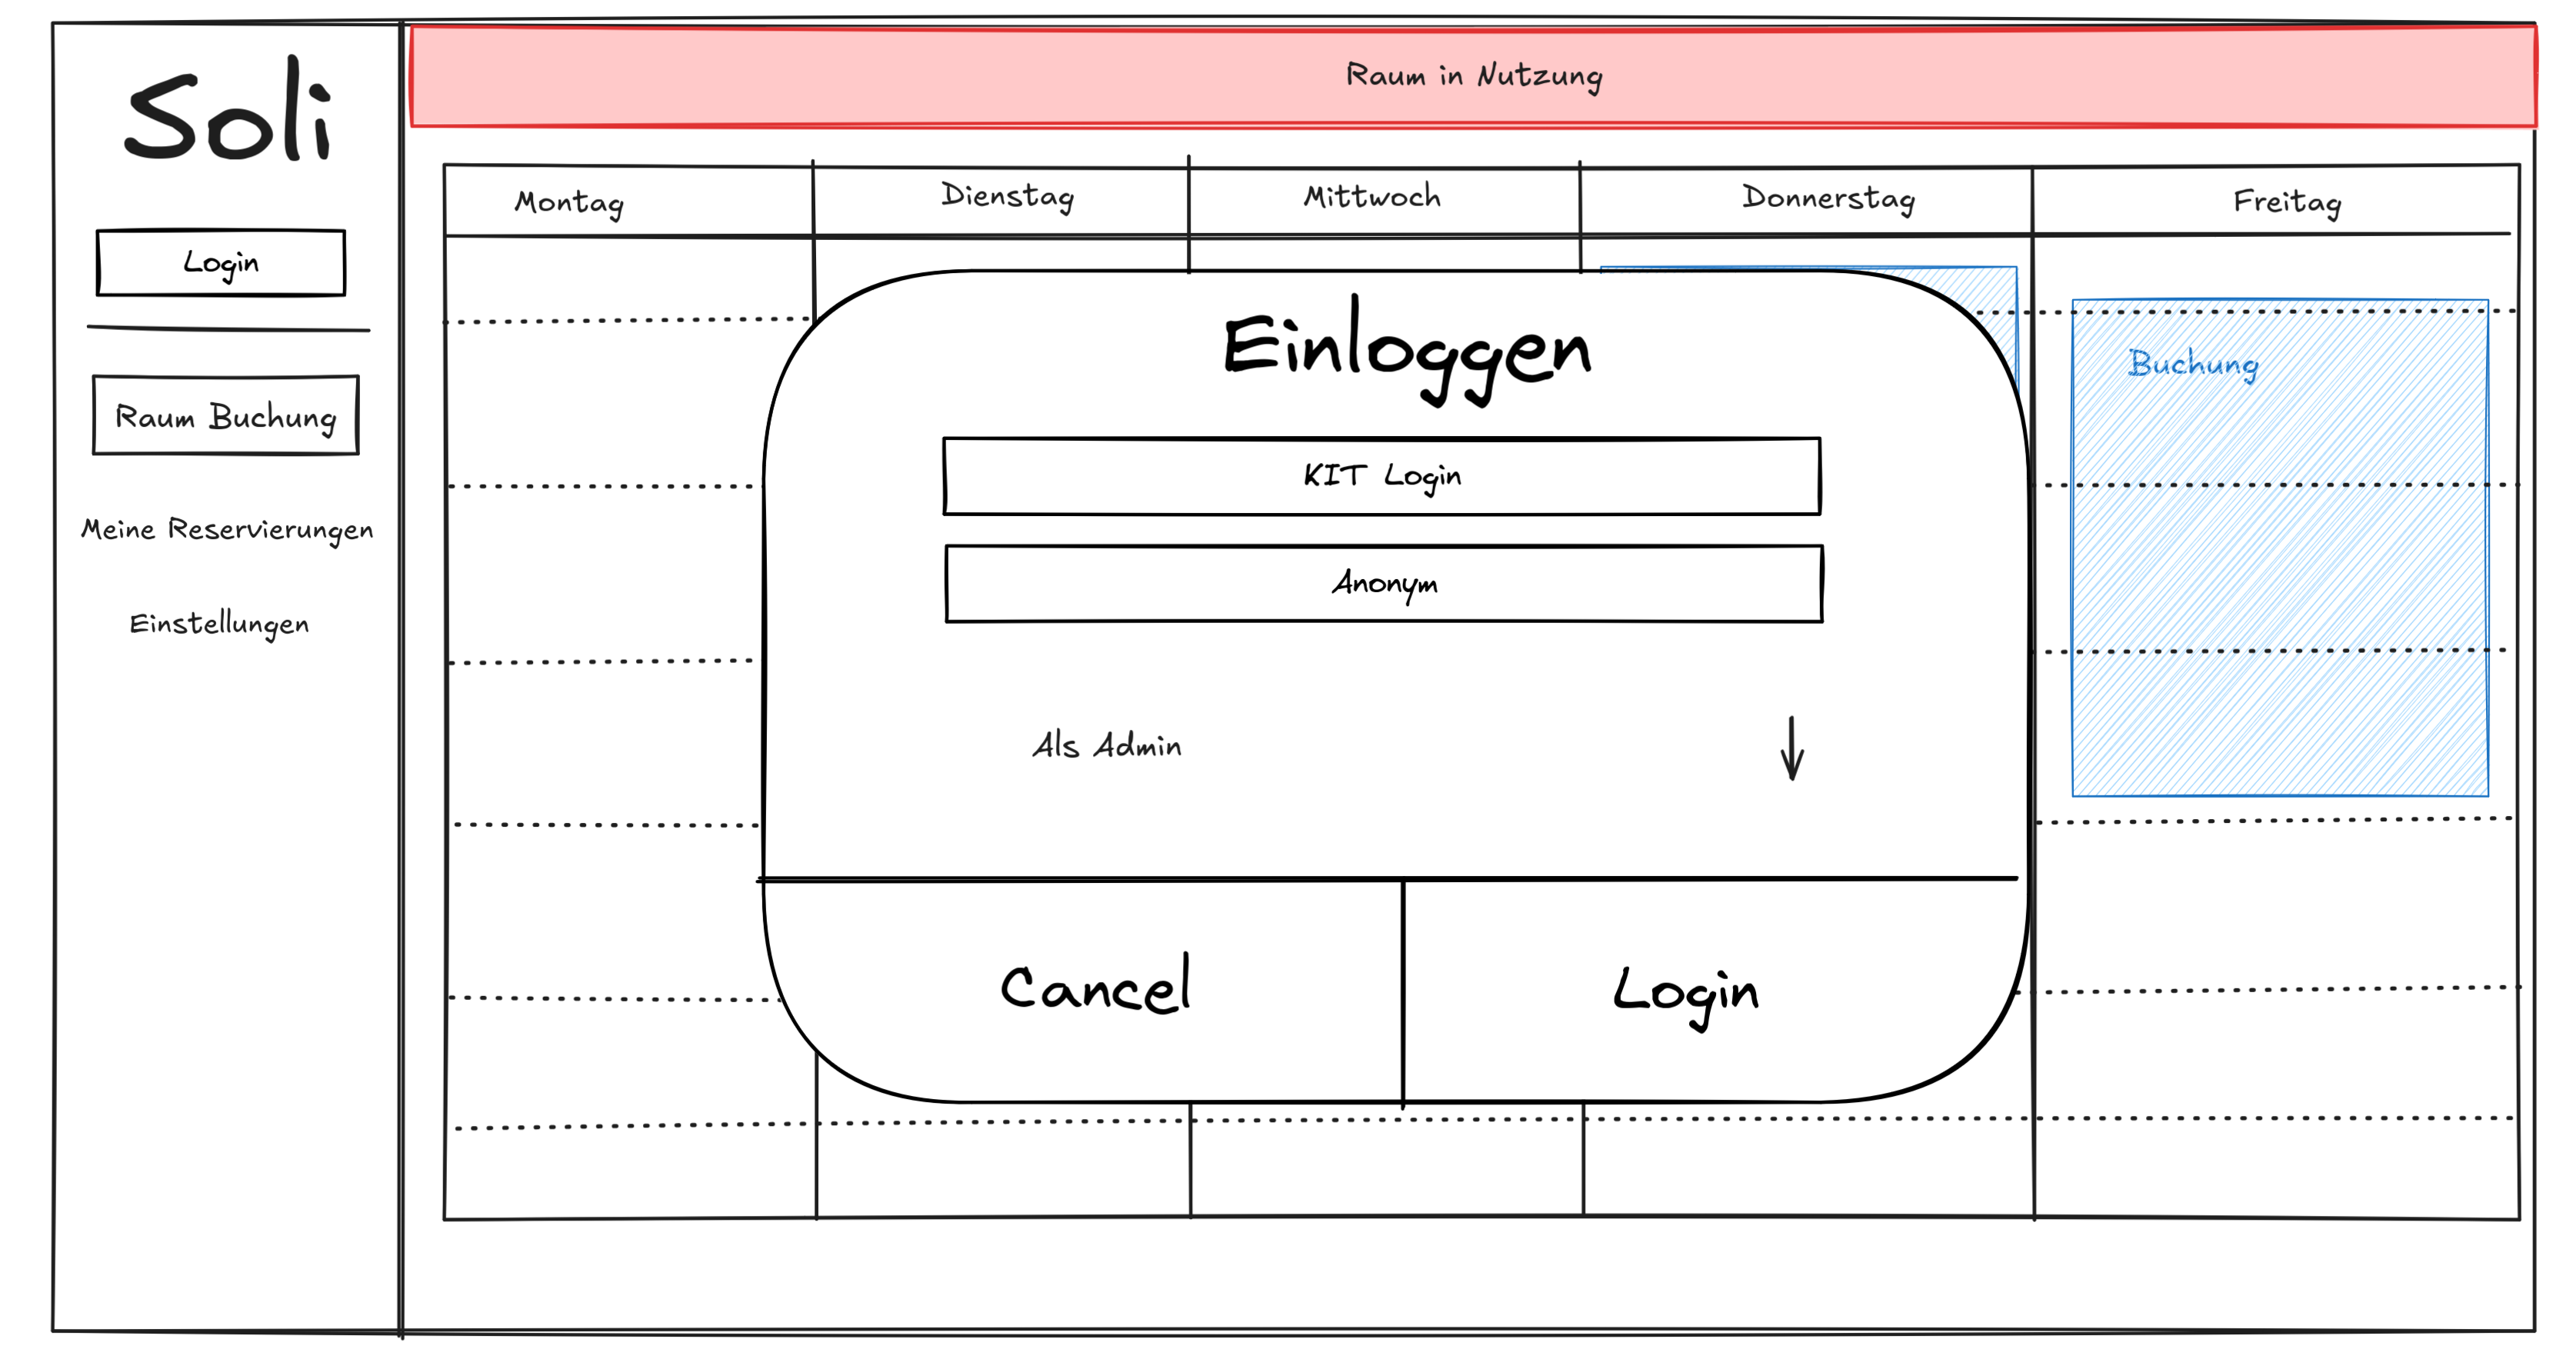
\includegraphics[width=\textwidth]{figures/mockup/auth_login}
    \caption{Anmeldungsseite}
    \label{fig:login}
\end{figure}
\clearpage

\begin{figure}[ht]
    \centering
    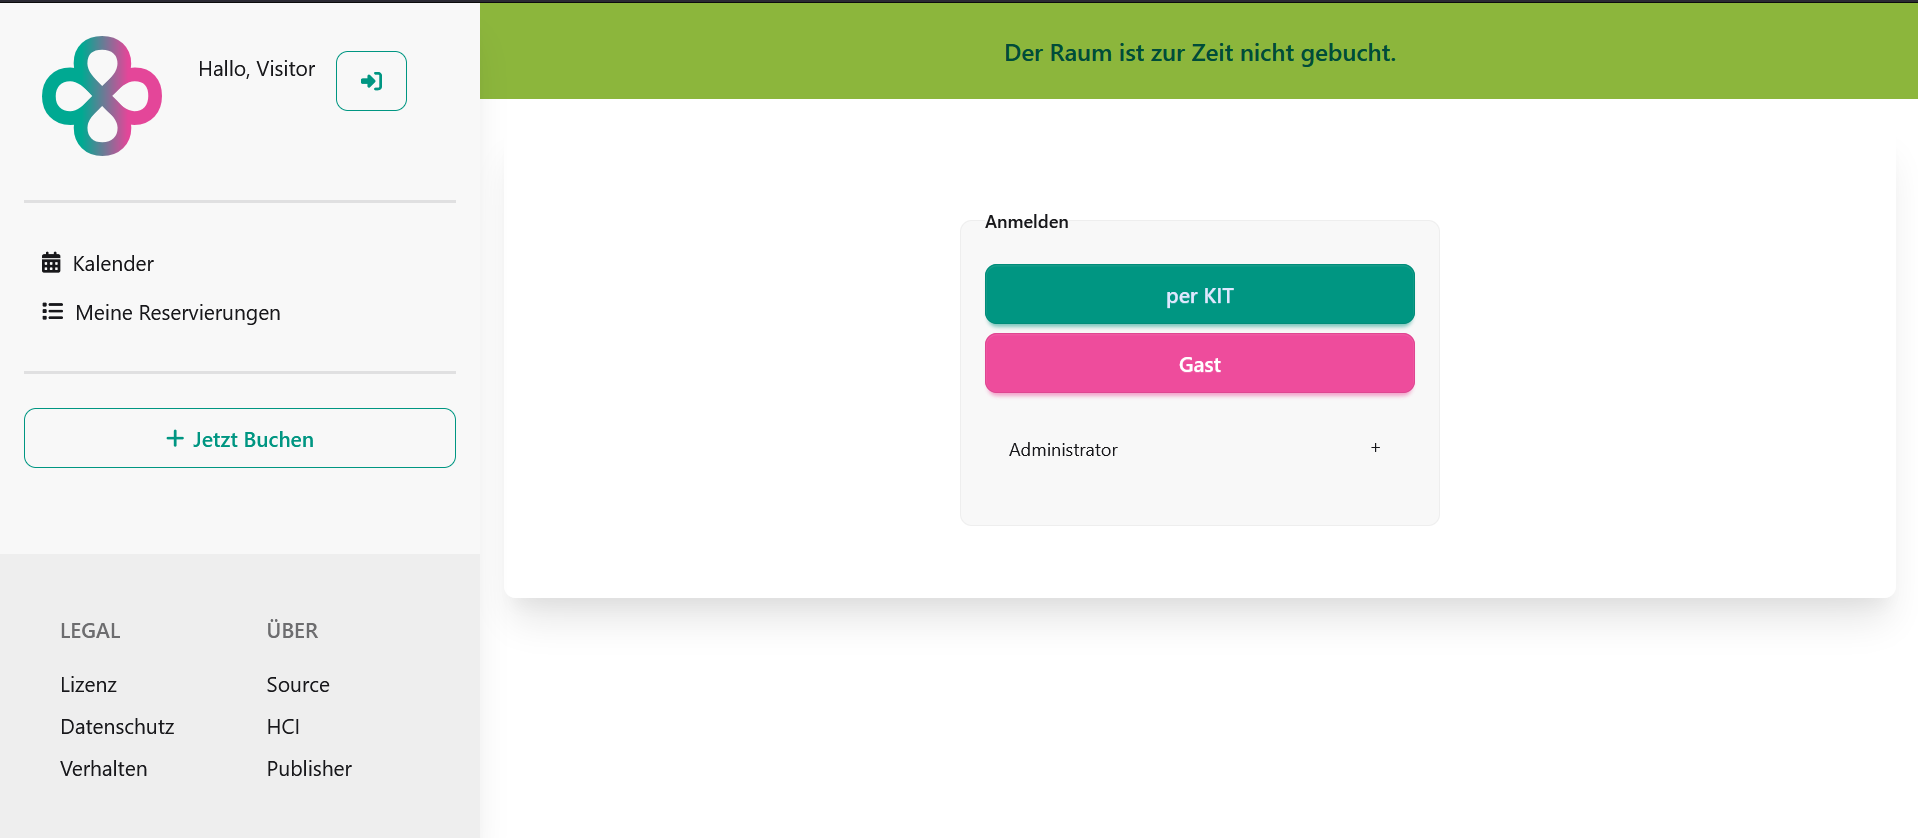
\includegraphics[width=\textwidth]{figures/impl-views/login_light}
    \caption{Implementierung: Anmeldungsseite}
    \label{fig:impl-login}
\end{figure}
\clearpage

Sind Nutzende eingeloggt und belegen den Raum,
so wird ihnen die in Abbildung \ref{fig:checkout} dargestellte Ansicht angezeigt.
Hier können Nutzende den Raum wieder über den Quick-Checkout-Button freigeben.

Die Implementierung davon ist in \ref{fig:impl-checkout} zu sehen.


Ziel dieser Ansicht ist es, Nutzenden das frühe Freigeben des Raumes ohne unnötigen Mehraufwand zu ermöglichen.
\begin{figure}[ht]
    \centering
    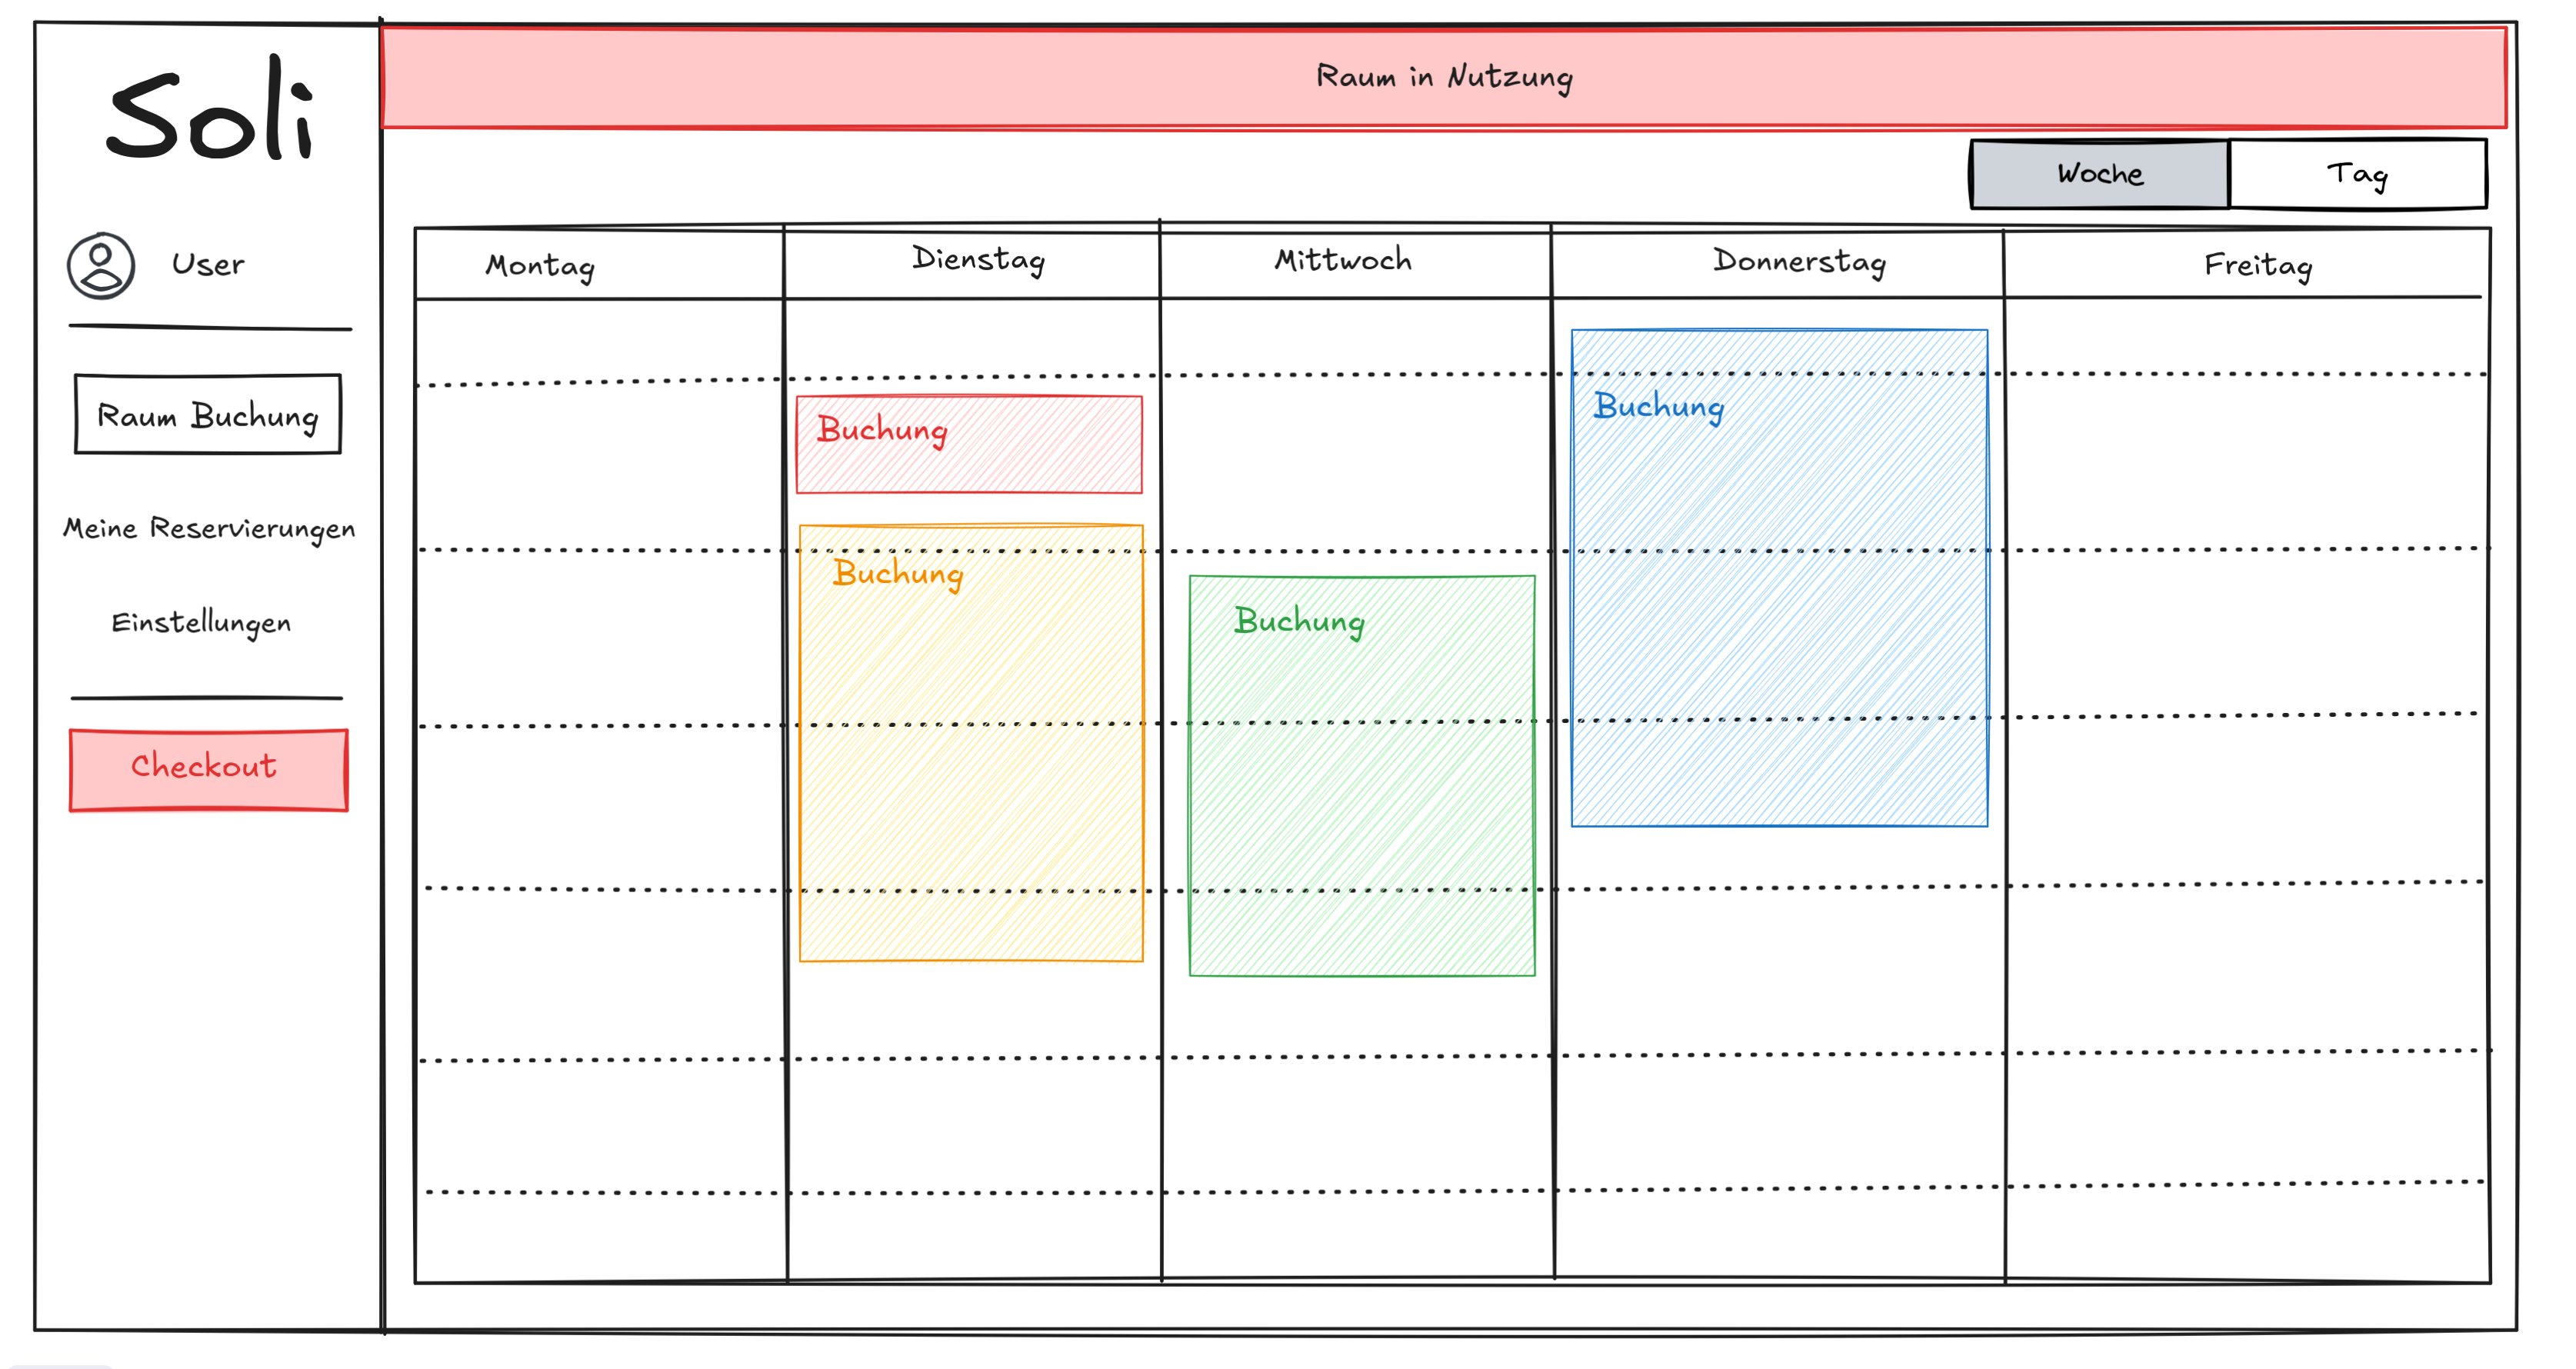
\includegraphics[width=\textwidth]{figures/mockup/calendar_checkout}
    \caption{Quick Checkout}
    \label{fig:checkout}
\end{figure}
\clearpage

\begin{figure}[ht]
    \centering
    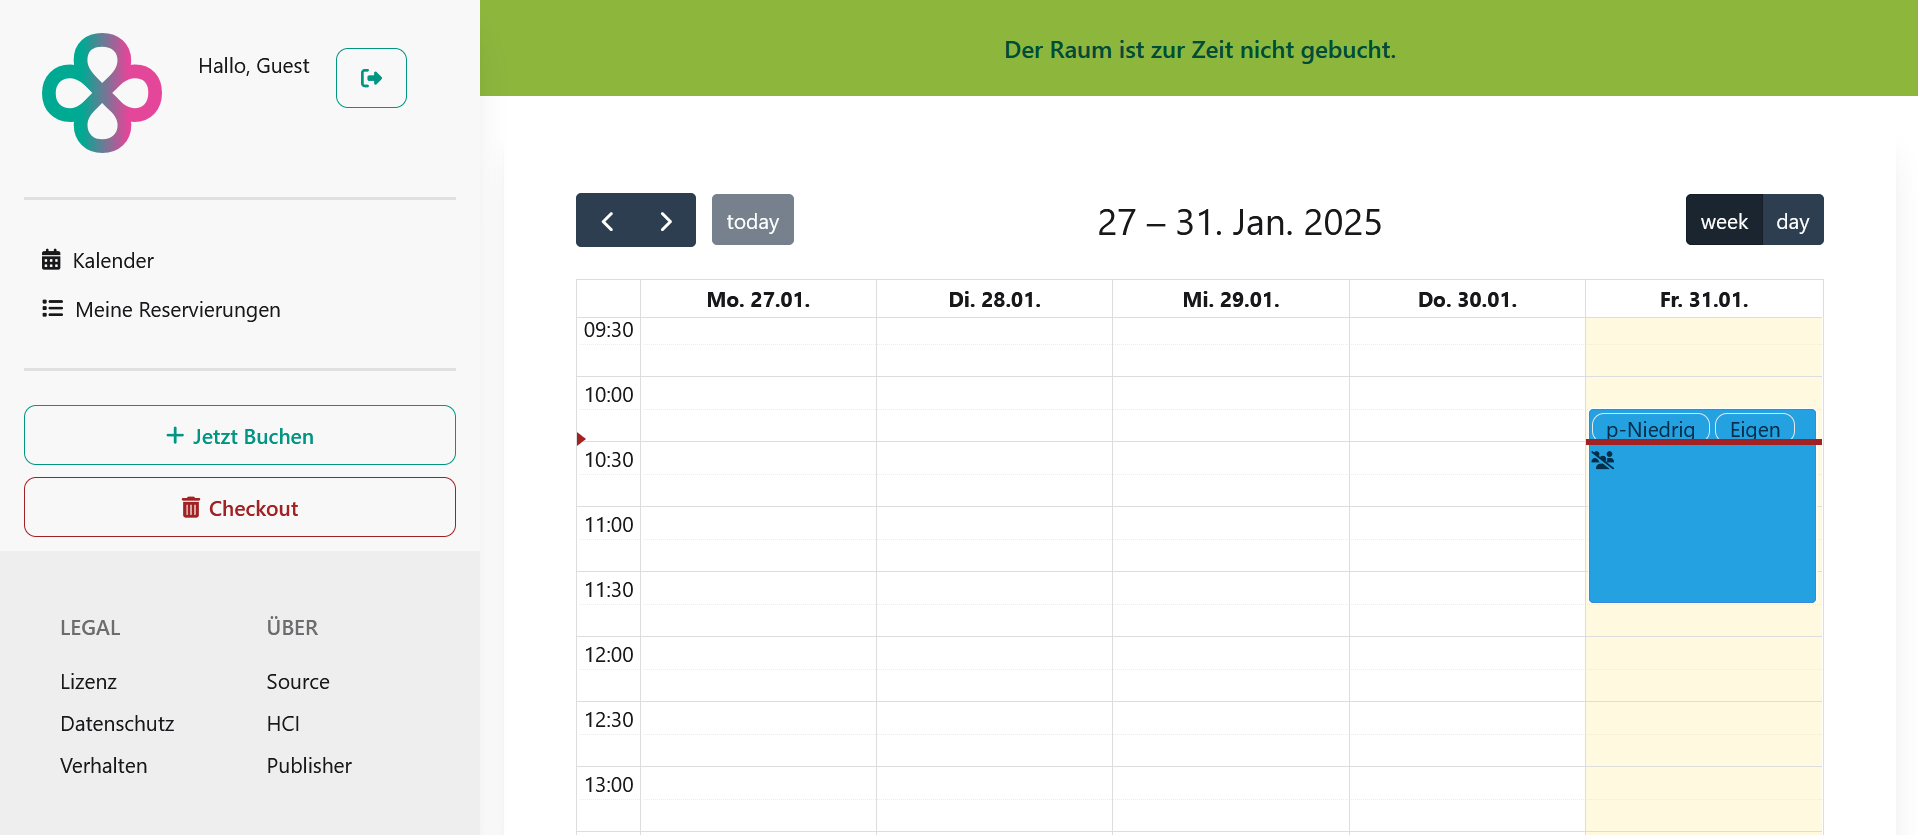
\includegraphics[width=\textwidth]{figures/impl-views/check_out_button_light}
    \caption{Implementierung: Quick Checkout}
    \label{fig:impl-checkout}
\end{figure}
\clearpage


\section{Terminübersicht}
Nutzende, die eine Buchung vorgenommen haben, können diese in der Terminübersicht,
die in Abbildung \ref{fig:overview} dargestellt ist, einsehen und verwalten.

Die Implementierung der Terminübersicht ist in \ref{fig:impl-overview} zu sehen und die der Terminansicht in \ref{fig:impl-calendarviewbooking}.

\begin{figure}[ht]
    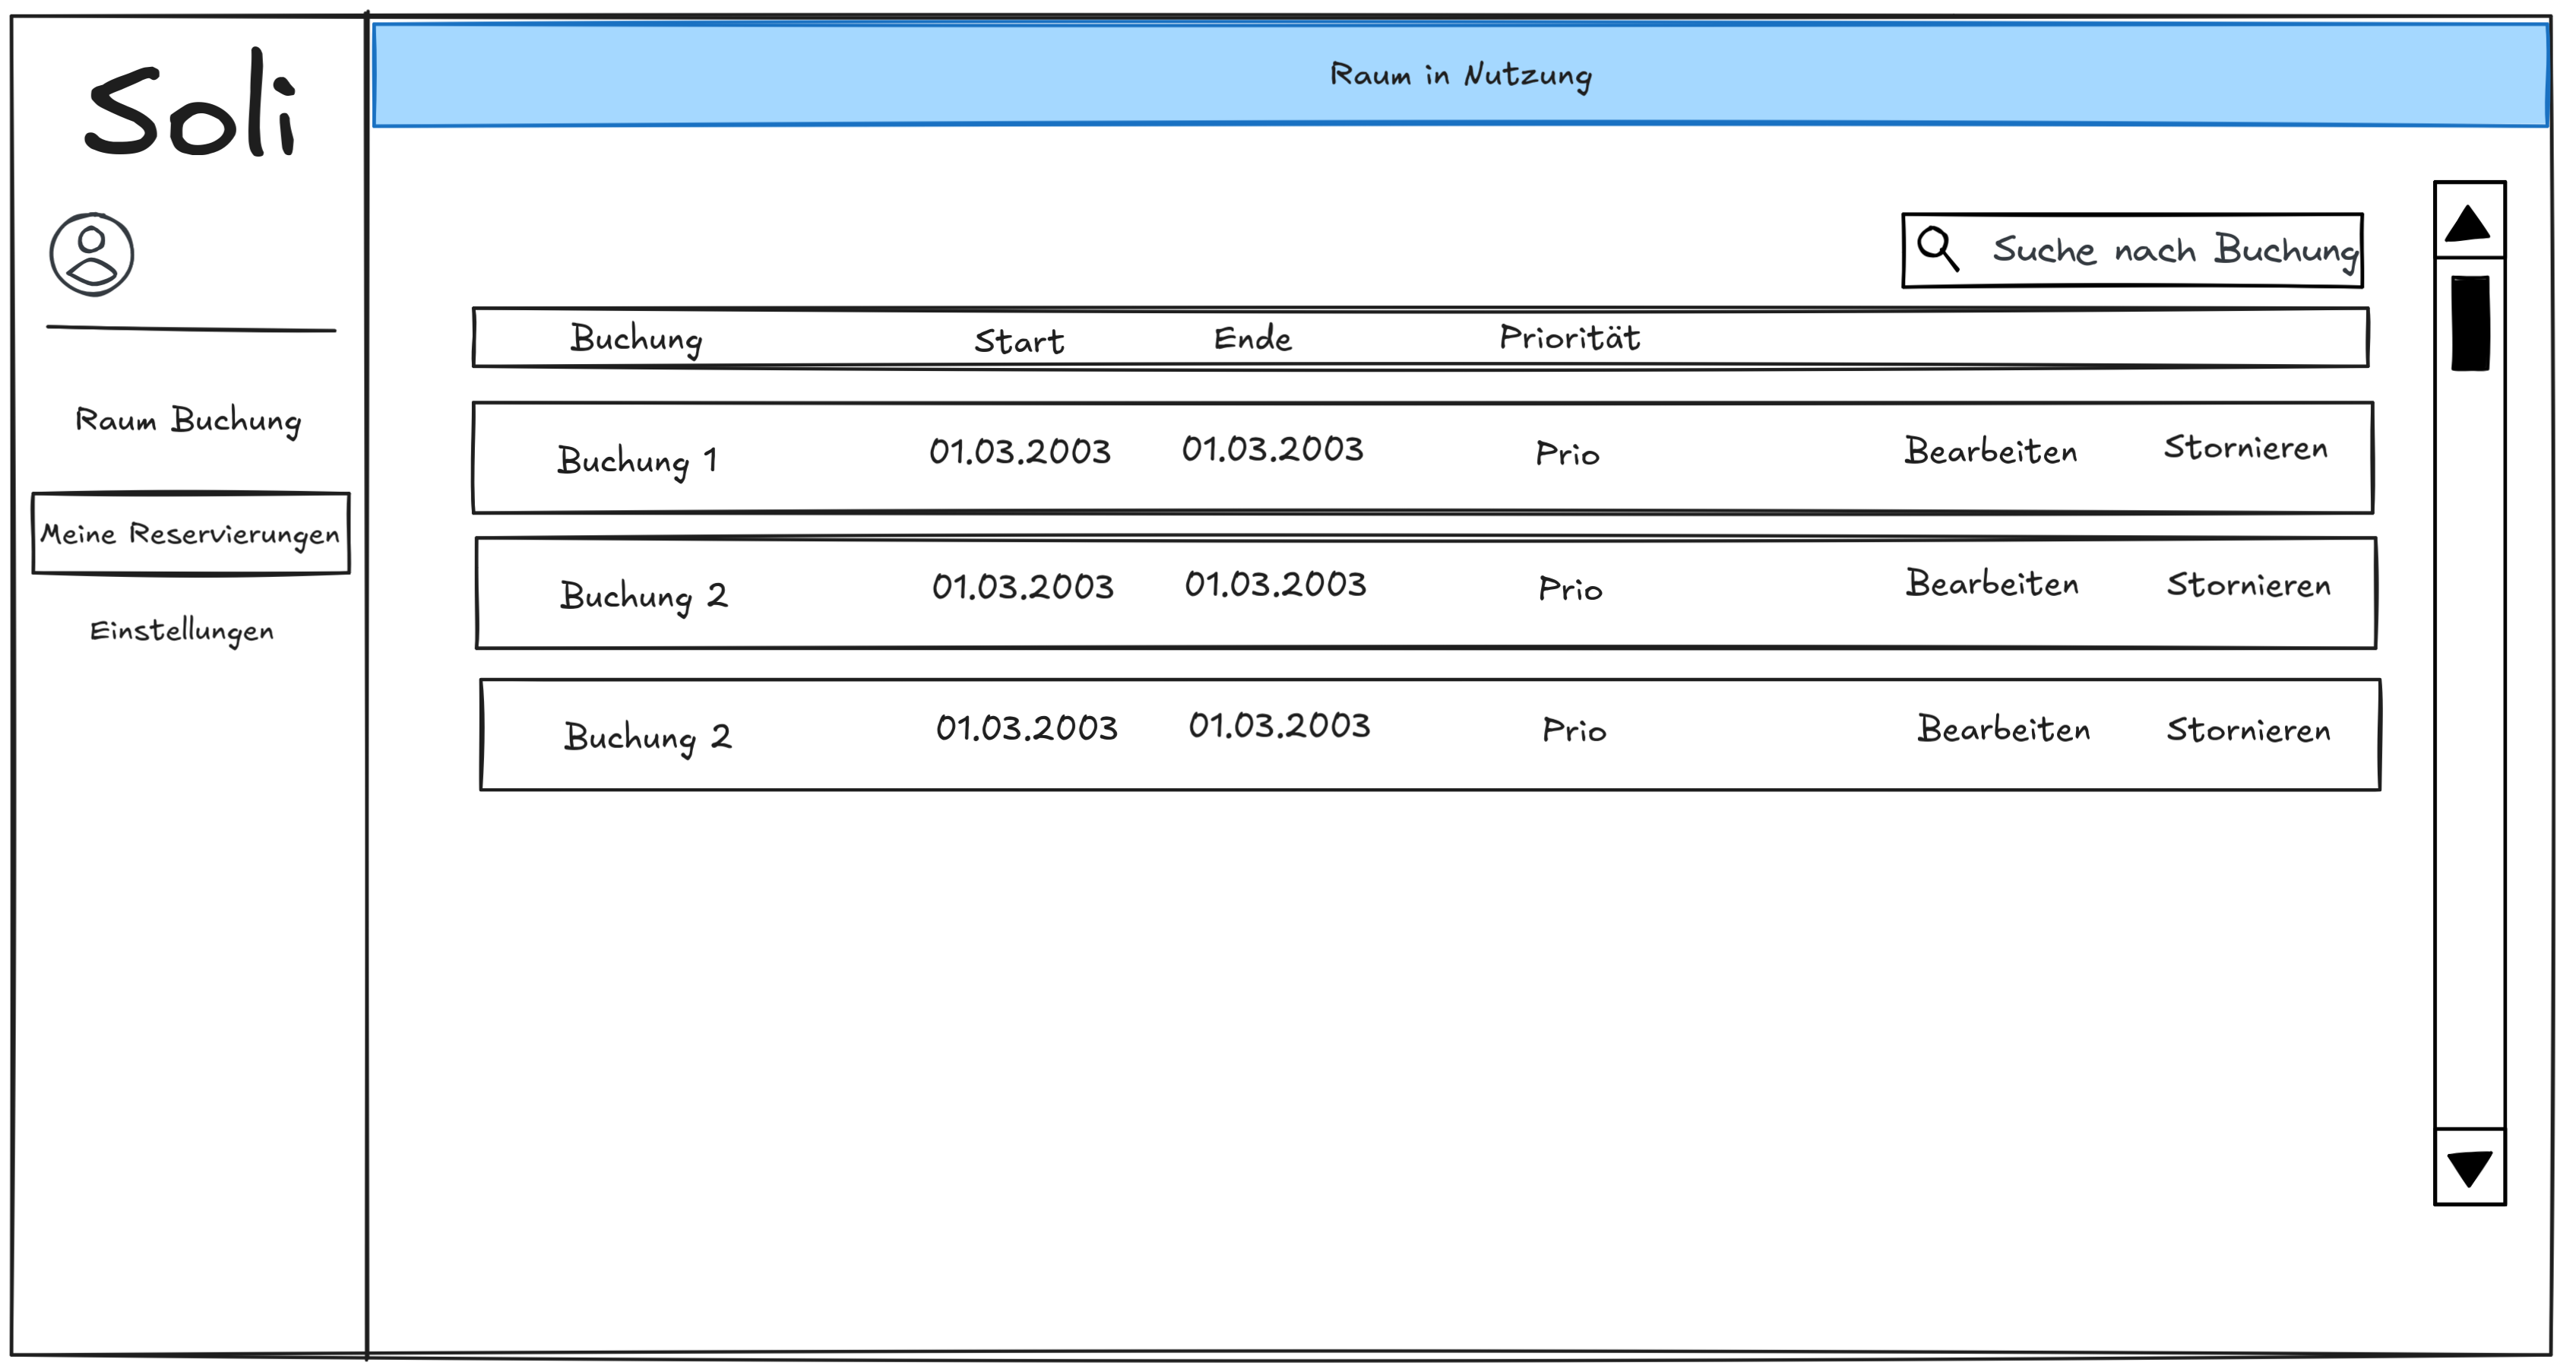
\includegraphics[width=\textwidth]{figures/mockup/bookings_list}
    \caption{Reservierungsübersicht}
    \label{fig:overview}
\end{figure}
\begin{figure}[ht]
    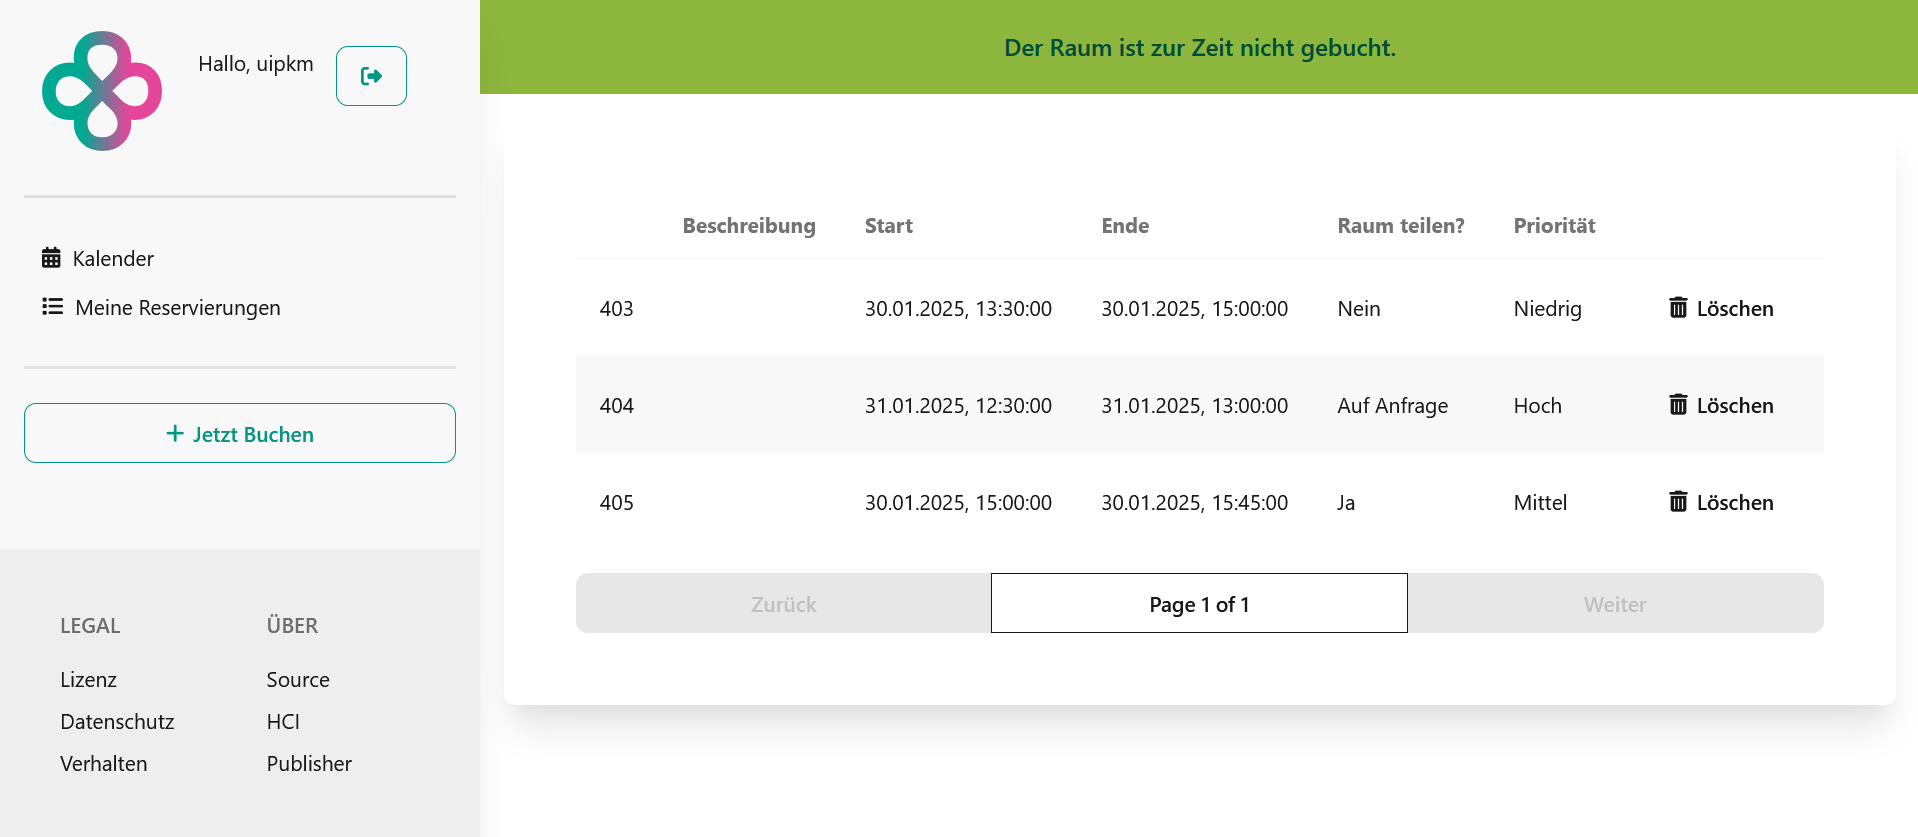
\includegraphics[width=\textwidth]{figures/impl-views/bookings_list_light}
    \caption{Implementierung: Reservierungsübersicht}
    \label{fig:impl-overview}
\end{figure}
\clearpage
\begin{figure}
    \centering
    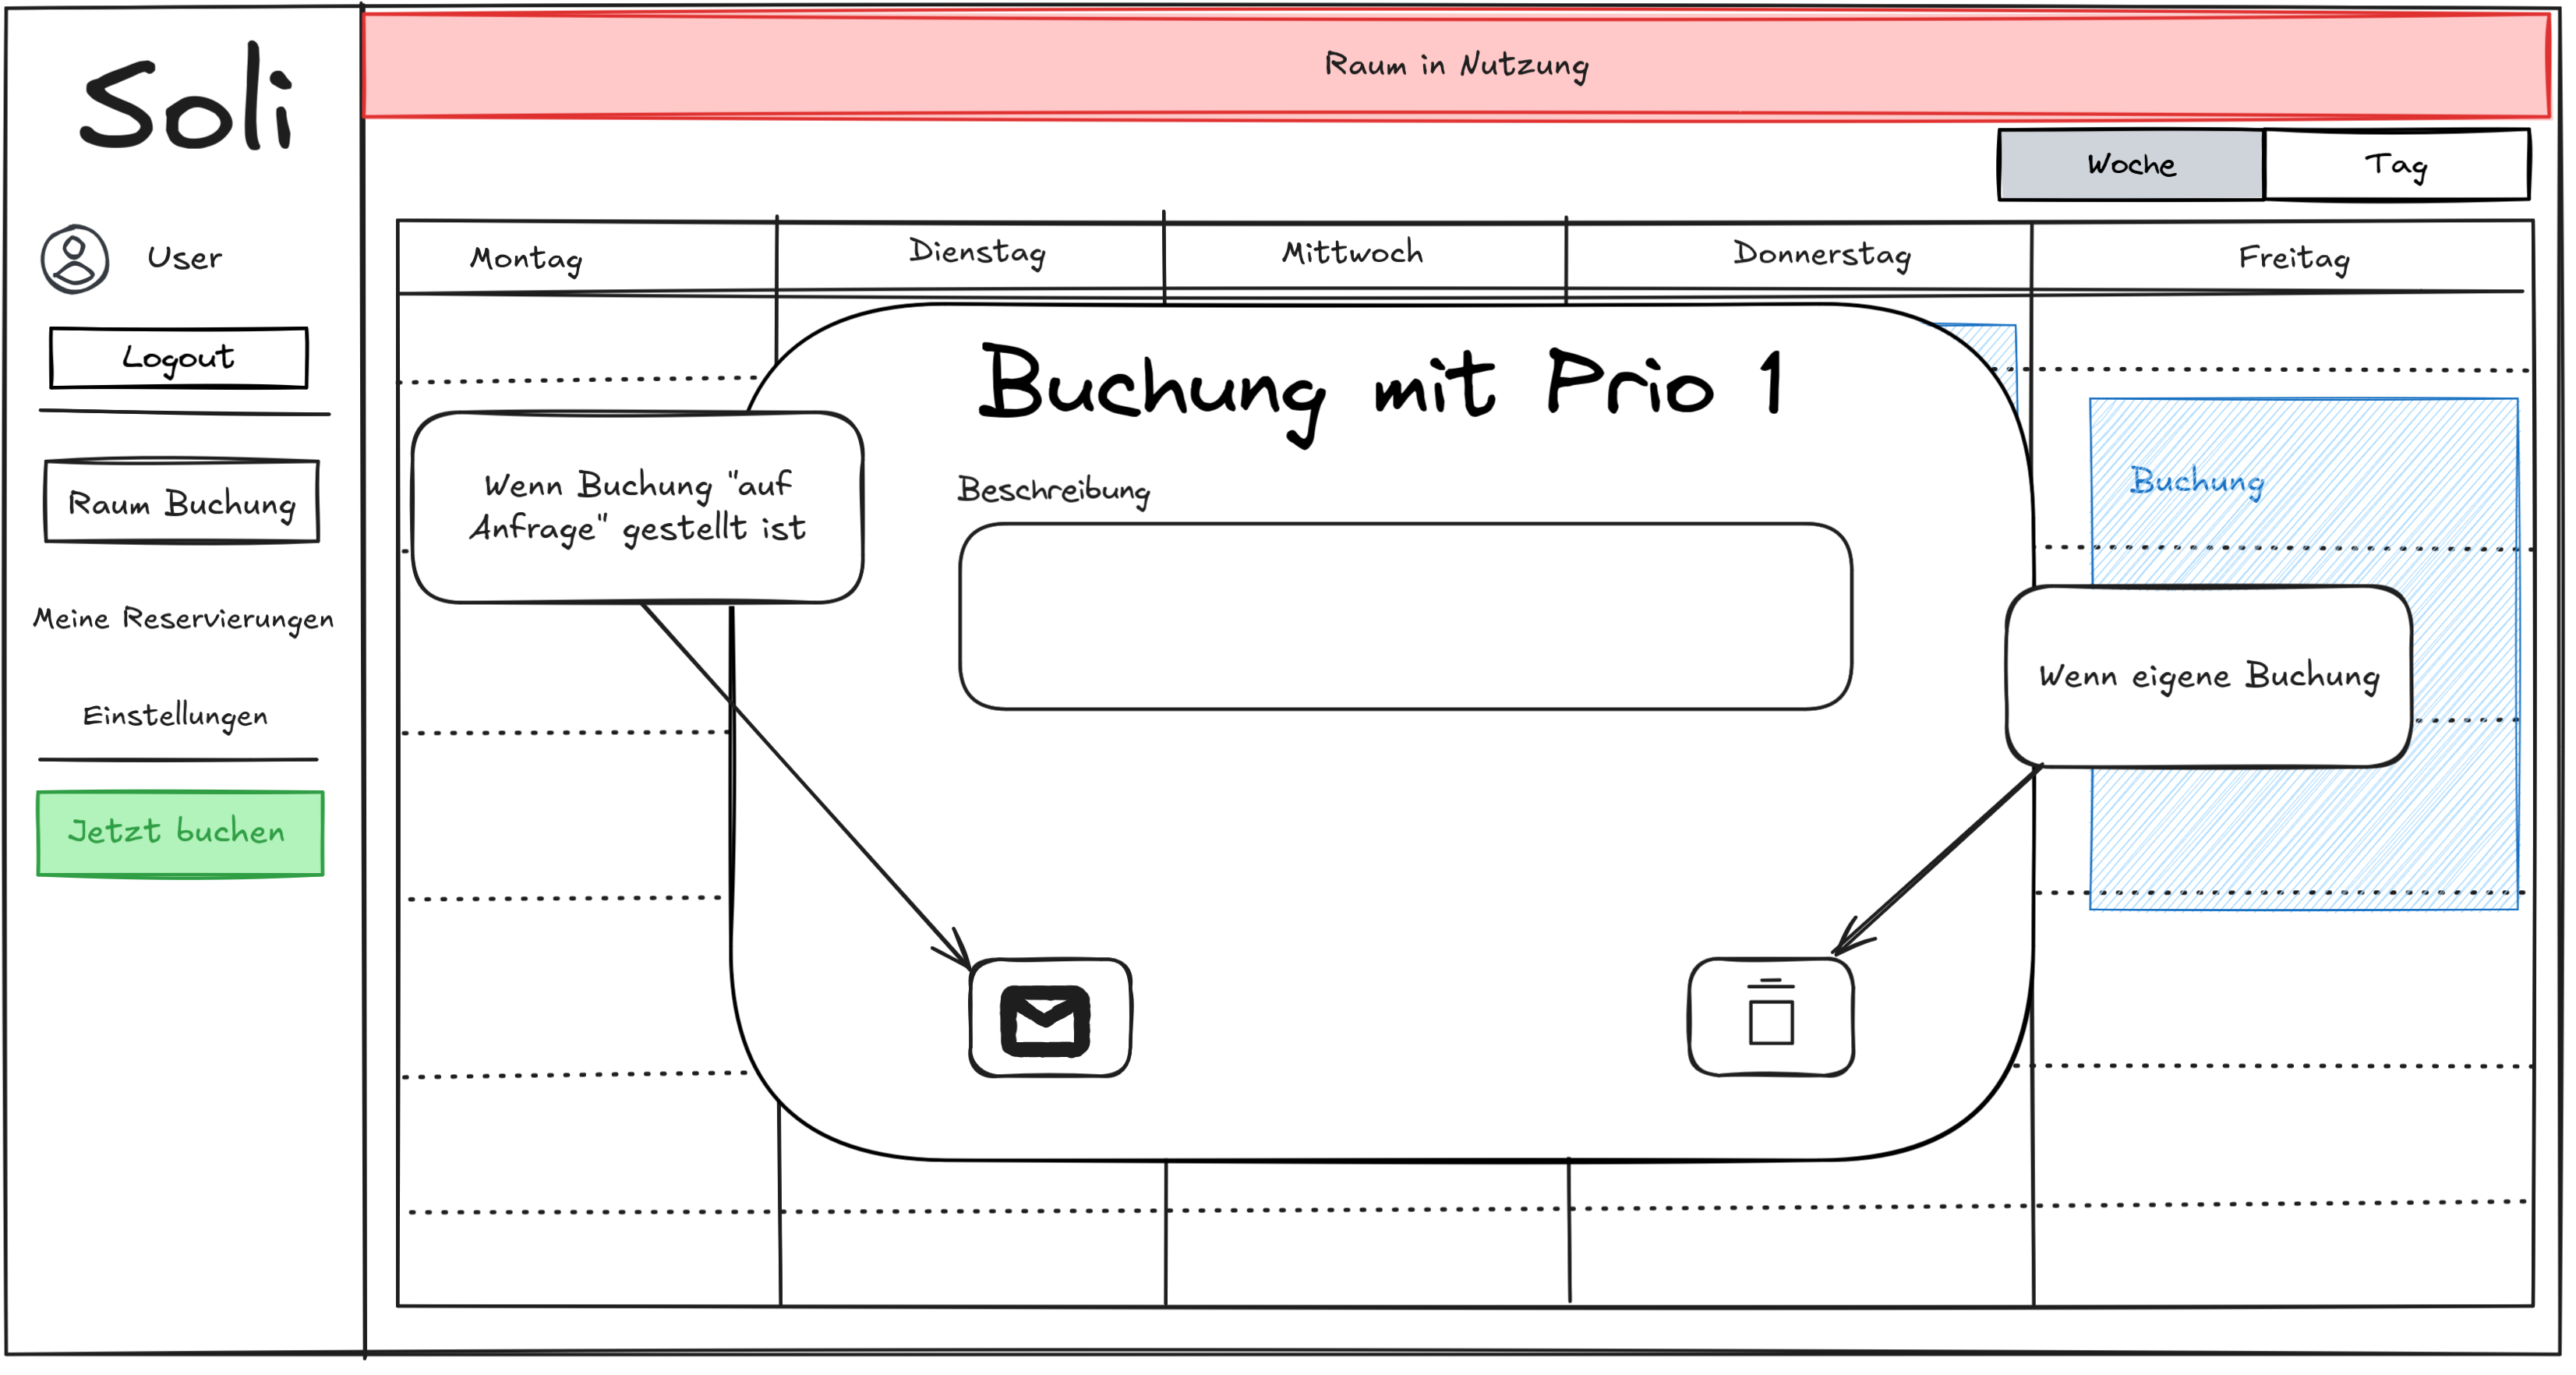
\includegraphics[width=\textwidth]{figures/mockup/bookings_single}
    \caption{Reserverierung im Kalender}
    \label{fig:calendarviewbooking}
\end{figure}
\begin{figure}
    \centering
    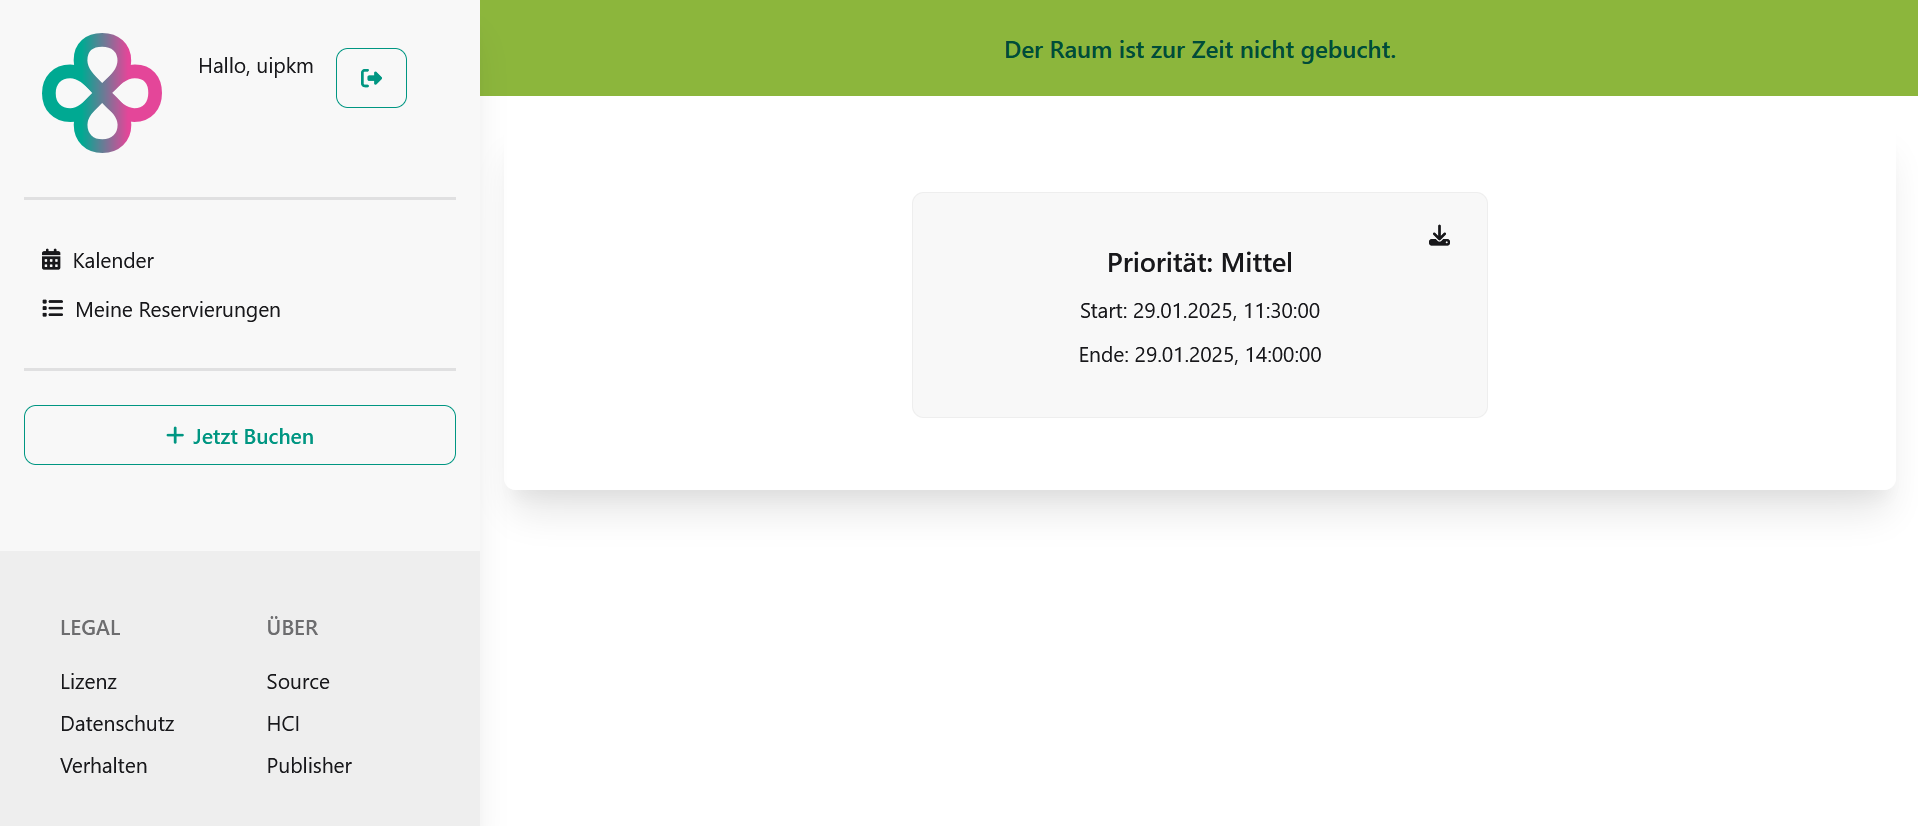
\includegraphics[width=\textwidth]{figures/impl-views/view_booking_light}
    \caption{Implementierung: Reserverierung im Kalender}
    \label{fig:impl-calendarviewbooking}
\end{figure}
\clearpage


\section{Adminstration}
Ein/e Administrator*in hat die Möglichkeit, über die Benutzeradministrationsoberfläche, die in Abbildung \ref{fig:adminuser} dargestellt ist, Nutzende einzusehen und zu verwalten.

Die Implementierung der Kontenliste ist in \ref{fig:impl-adminuser} dargestellt.

\begin{figure}[ht]
    \centering
    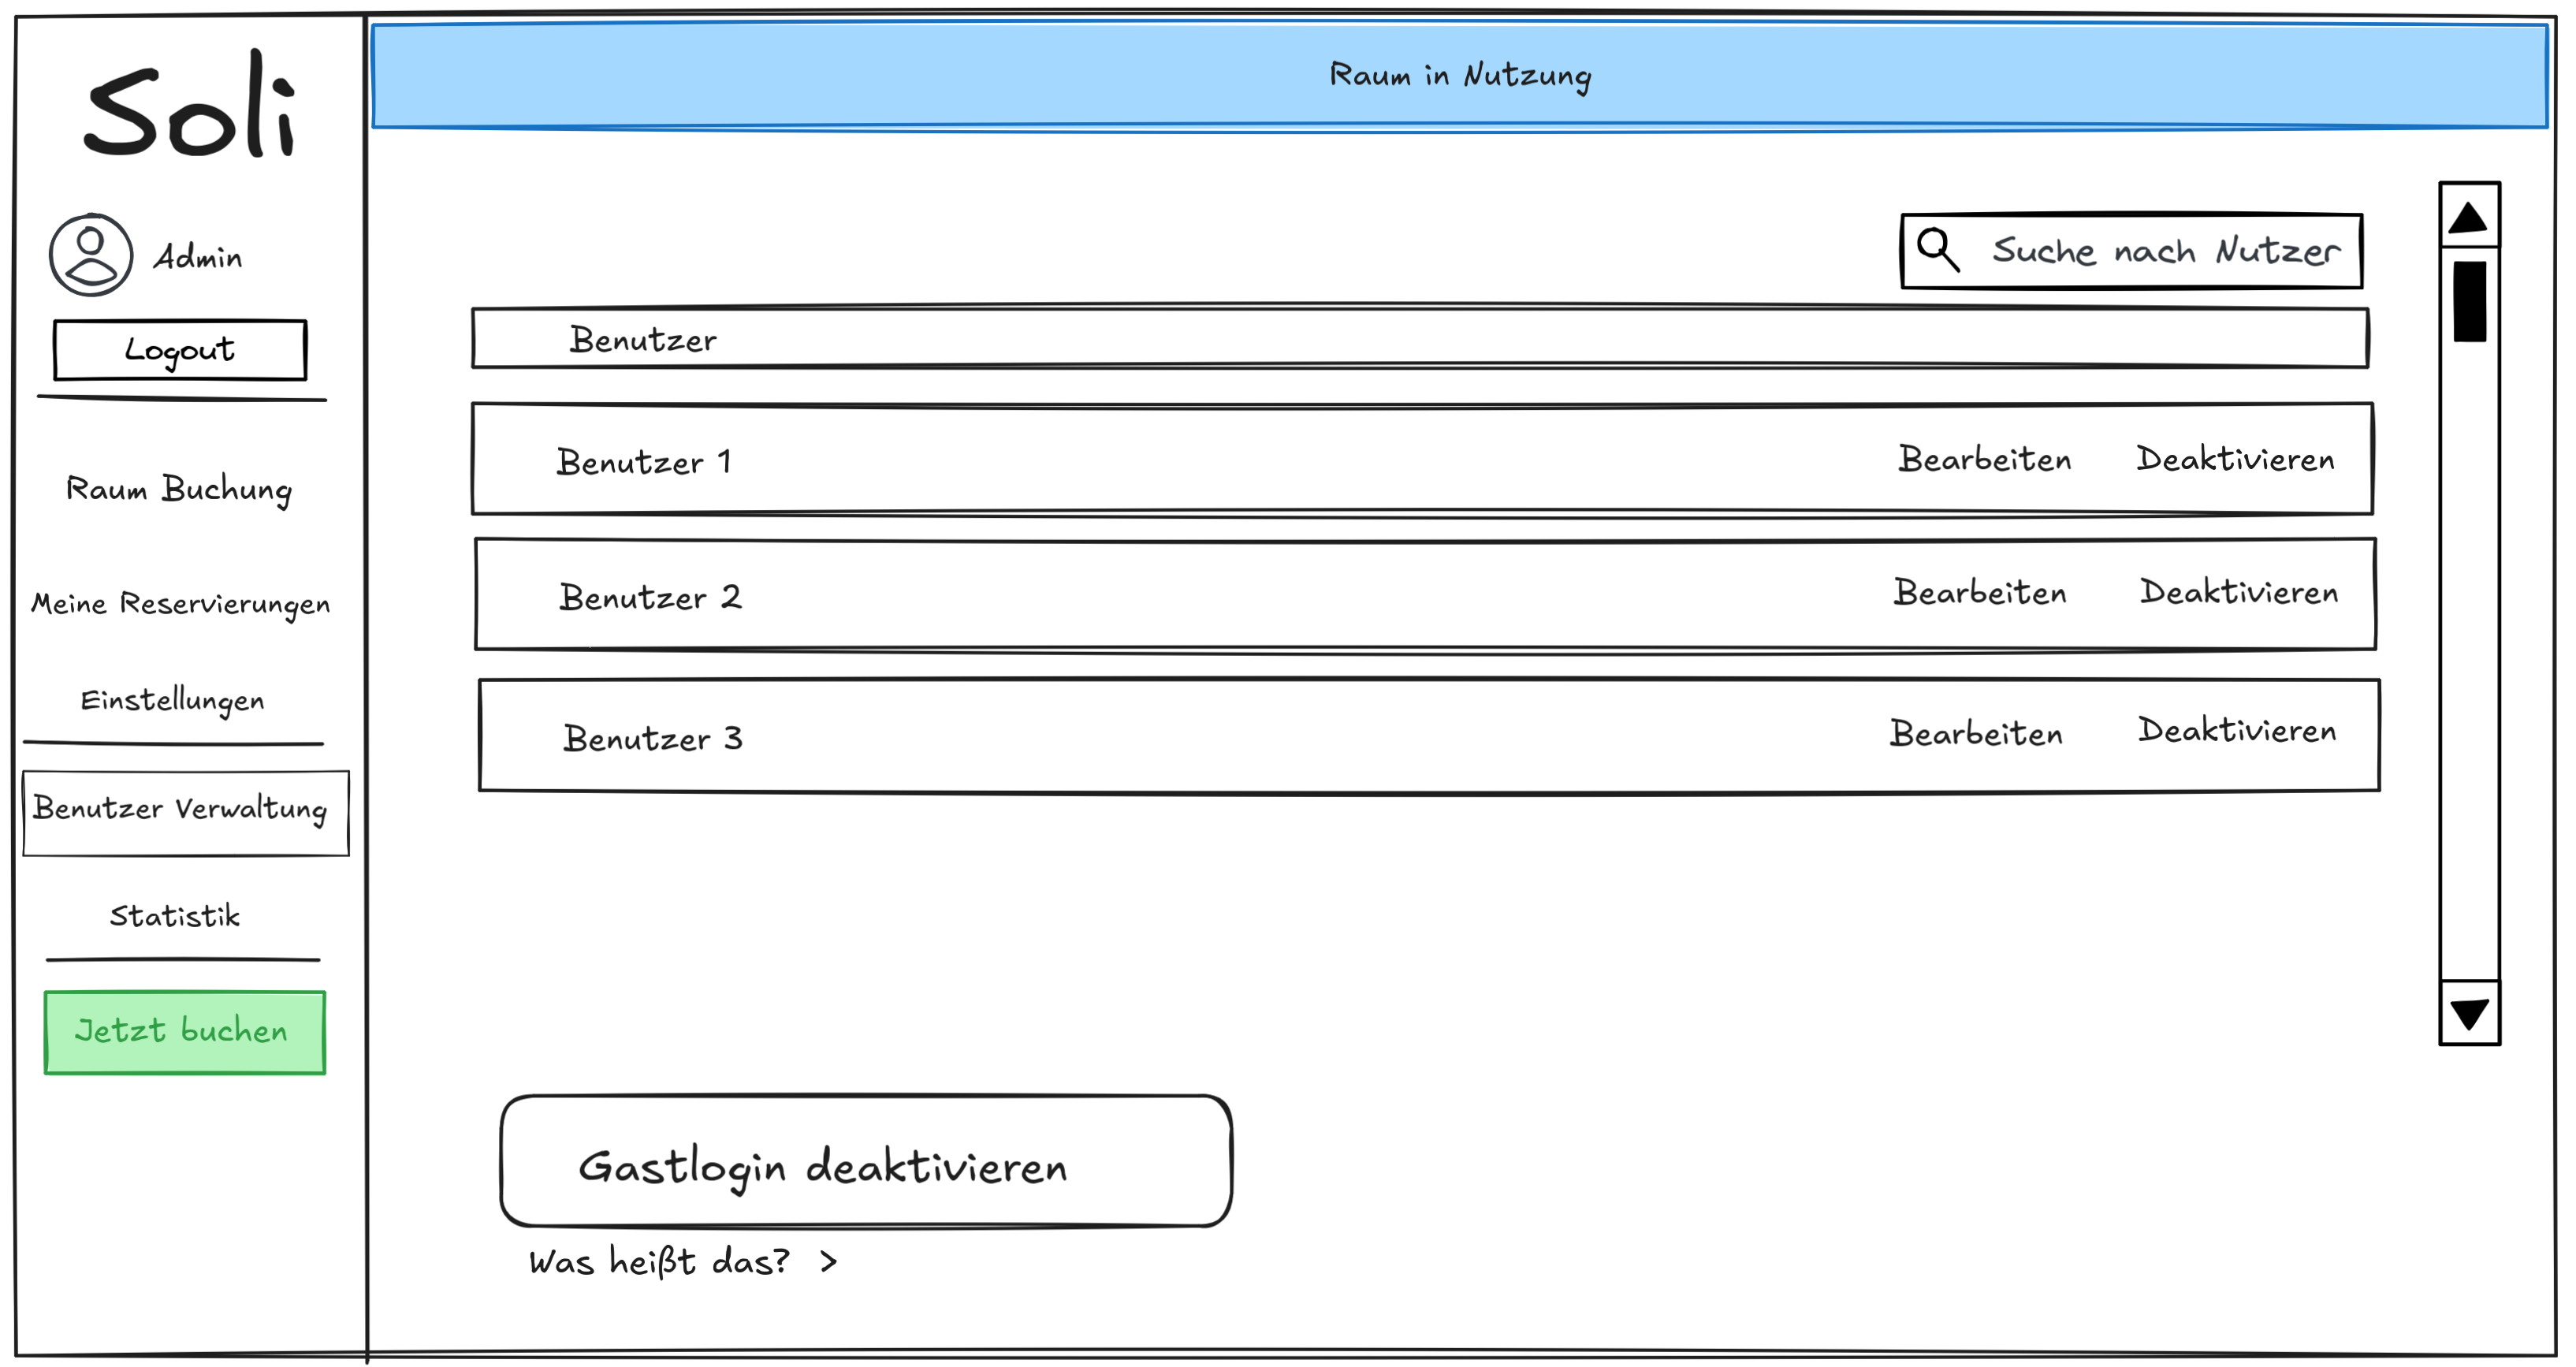
\includegraphics[width=\textwidth]{figures/mockup/admin_users}
    \caption{Benutzeradminstrationsoberfläche}
    \label{fig:adminuser}
\end{figure}
\begin{figure}[ht]
    \centering
    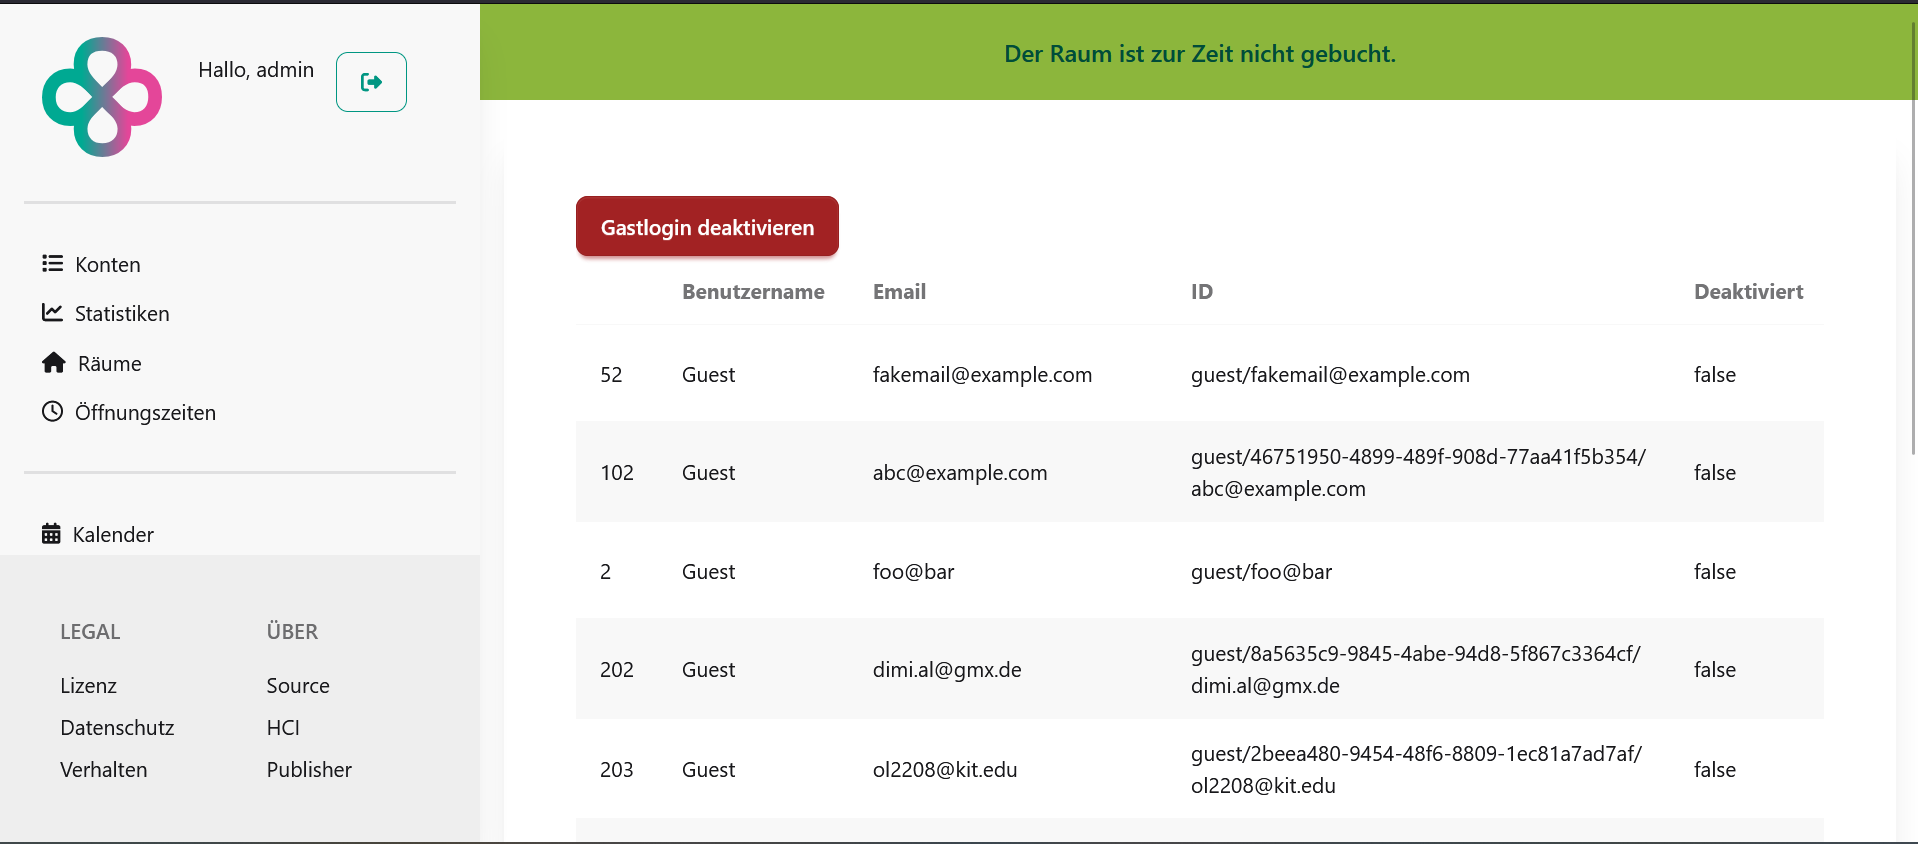
\includegraphics[width=\textwidth]{figures/impl-views/user_list_light}
    \caption{Implementierung: Benutzeradminstrationsoberfläche}
    \label{fig:impl-adminuser}
\end{figure}
\clearpage

Die Funktionalität der einstellbaren Öffnungszeiten für einen Raum, welche nur von Administrator*innen genutzt werden kann
ist in seiner implementierten Form in \ref{fig:impl-adminopeninghours_config} zu sehen.

Die implementierte Visualisierung der Öffnungszeiten in der \textit{Kalender} Ansicht in \ref{fig:impl-adminopeninghours} zu sehen ist.

\begin{figure}[ht]
    \centering
    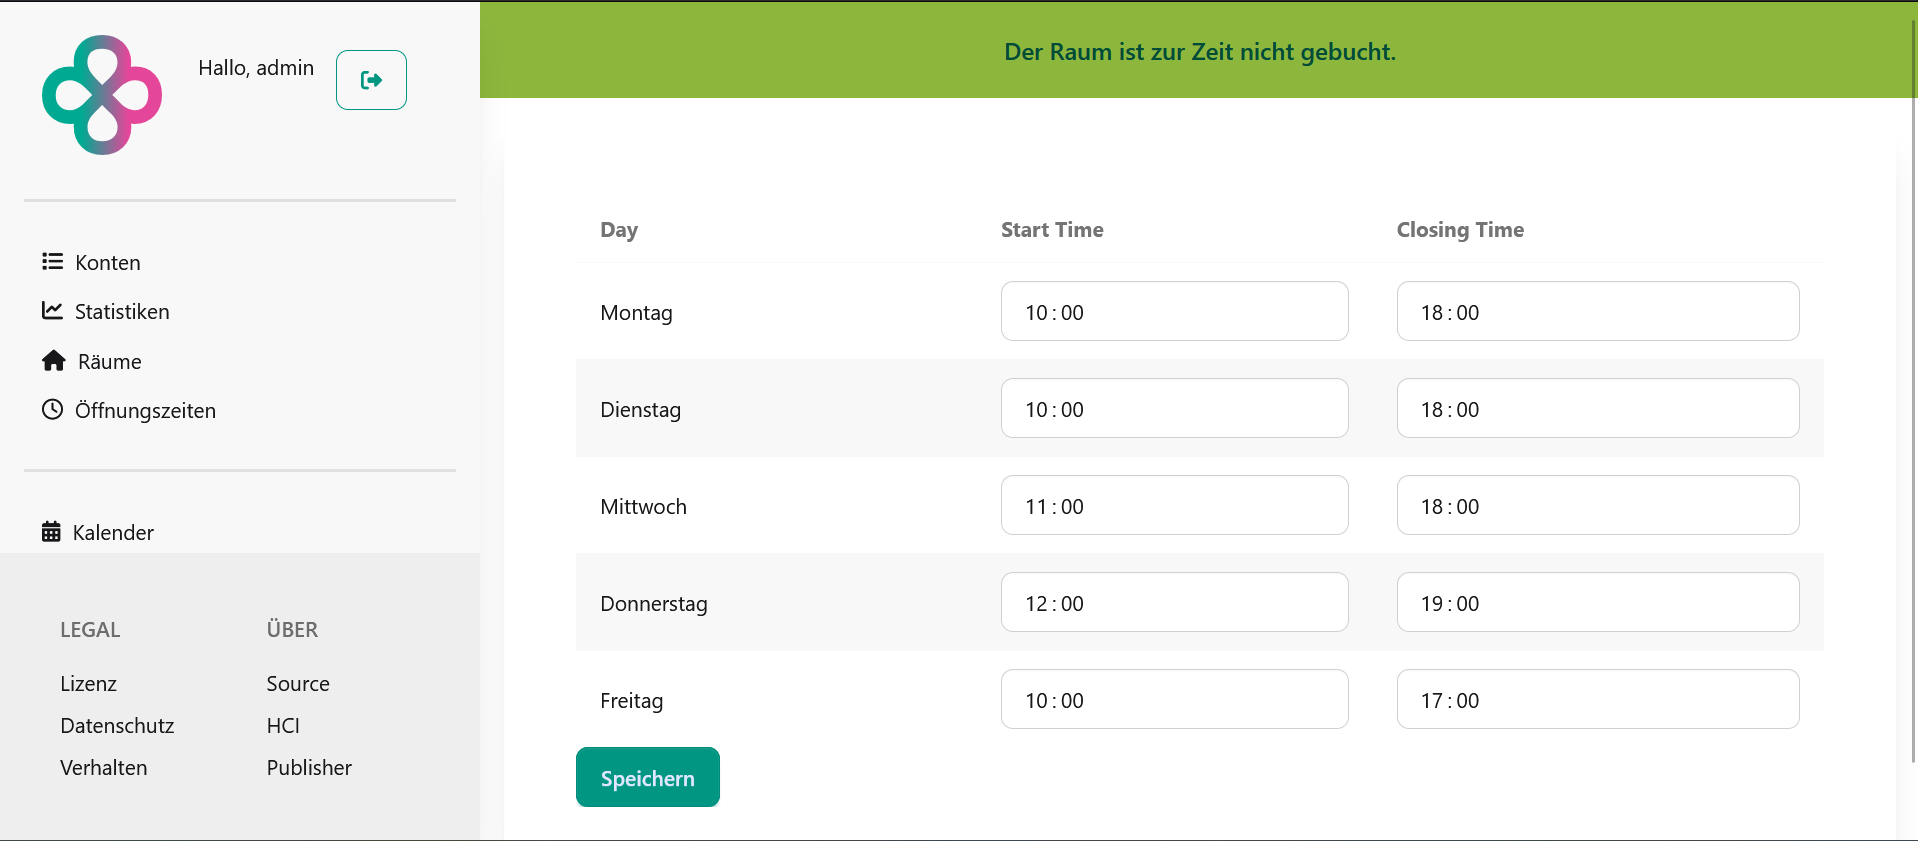
\includegraphics[width=\textwidth]{figures/impl-views/set_opening_hours_light}
    \caption{Implementierung: Konfiguration}
    \label{fig:impl-adminopeninghours_config}
\end{figure}
\begin{figure}[ht]
    \centering
    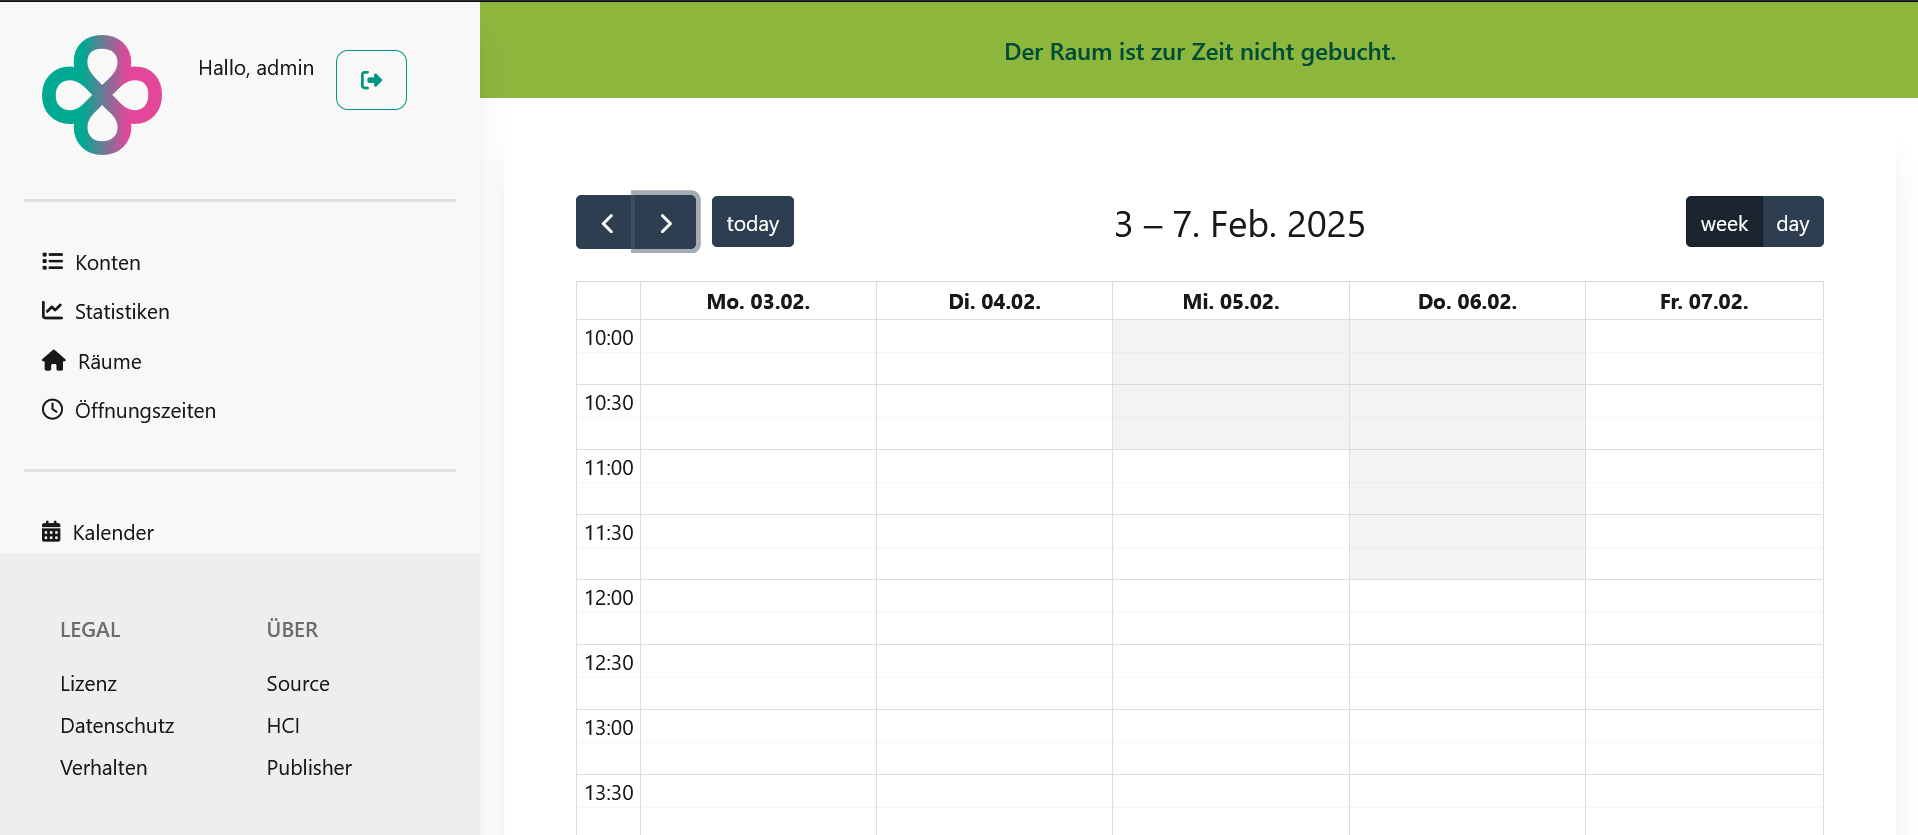
\includegraphics[width=\textwidth]{figures/impl-views/opening_hours_calendar_light}
    \caption{Implementierung: Visualisierung der Öffnungszeiten}
    \label{fig:impl-adminopeninghours}
\end{figure}
\clearpage

Die Implementierung des Wunschkriteriums einer Statistikansicht für ein/e Administrator*in ist in \ref{fig:impl-adminstatistic} zu sehen.

\begin{figure}[ht]
    \centering
    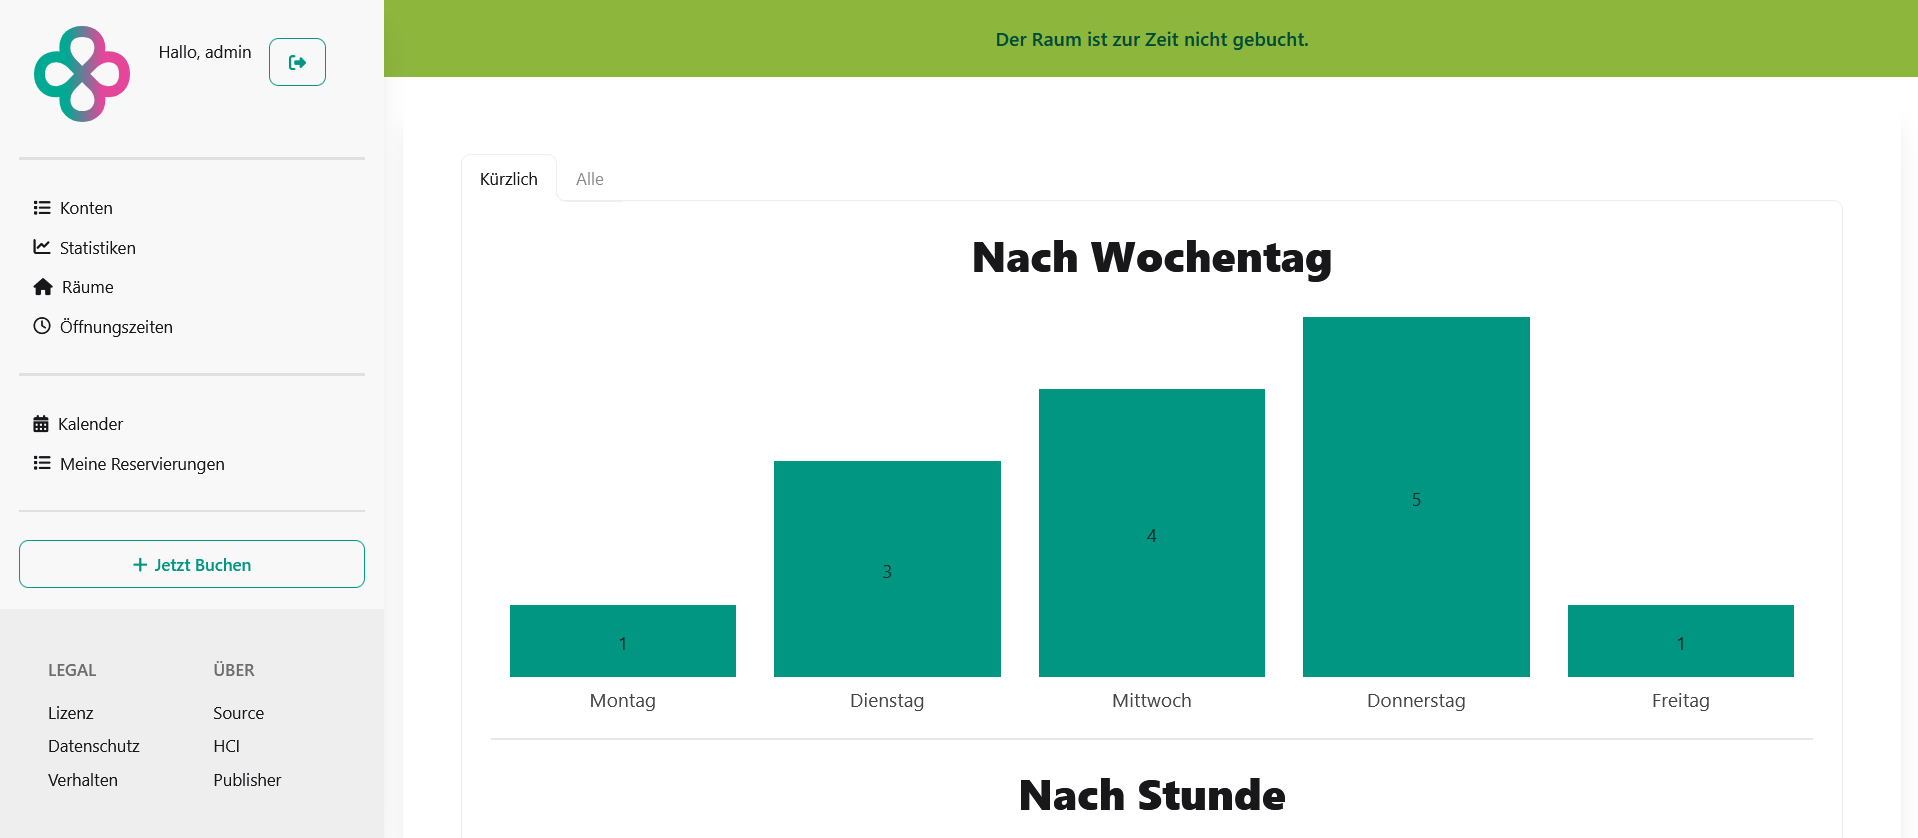
\includegraphics[width=\textwidth]{figures/impl-views/stats_light}
    \caption{Implementierung: Statistikansicht}
    \label{fig:impl-adminstatistic}
\end{figure}